\documentclass[11pt]{article}
\usepackage[mono=false]{libertinus}
\directlua{luaotfload.add_fallback("monofallback", {"DejaVu Sans Mono:mode=node;"})}
\setmonofont{JetBrainsMono Nerd Font}[
  SizeFeatures={Size=9},
  RawFeature={fallback=monofallback},
]
\usepackage{graphicx}
\usepackage{longtable}
\usepackage{booktabs}
\usepackage{wrapfig}
\usepackage{rotating}
\usepackage[normalem]{ulem}
\usepackage{amsmath}
\usepackage{amsthm}
\usepackage{capt-of}
\usepackage{hyperref}
\usepackage{amsthm}
\usepackage{nicematrix}
\usepackage{mathpartir}
\usepackage{mathtools}
\usepackage{parskip}
\usepackage{float}
\usepackage[margin=1in]{geometry}
\usepackage{tikz}
\usetikzlibrary{positioning,calc,decorations,automata,arrows.meta}
\usepackage{array}
\usepackage{multirow}
\usepackage{listings}
\usepackage{minted}
\newmintinline[lean]{lean4}{bgcolor=white}
\newminted[leancode]{lean4}{fontsize=\footnotesize}
\usepackage{caption}
\usepackage{subcaption}
\usepackage{stmaryrd}
\usepackage[backend=biber,sorting=ynt]{biblatex}
\usepackage{xpatch}
\usepackage{metavarsx}
\usepackage{pl-syntax}
\AtBeginDocument{%
  \renewcommand{\Coloneqq}{\mathrel{\Colon\mkern-1.2mu=}}%
  \renewcommand\doubleplus{\ensuremath{\mathbin{+\mkern-6mu+}}}
} % Needed since libertinus math doesn't have ::= as one glyph.
\usepackage{unicode-math}           % load after amsmath/mathtools
\setmathfont{Libertinus Math}

\addbibresource{pollux.bib}
\author{Matt Schwennesen}
\title{Pollux: Parser Compatibility Checking}
\date{}
\hypersetup{
 pdfauthor={Matt Schwennesen},
 pdftitle={Pollux},
 pdfkeywords={},
 pdfsubject={},
 pdflang={English}
}
\lstdefinelanguage{proto}{
  keywords={message,double,float,int32,int64,uint32,uint64,sint32,sint64,fixed32,fixed64,sfixed32,sfixed64,bool,string,bytes,oneof,enum}
}
\definecolor{codegreen}{rgb}{0,0.6,0}
\definecolor{codegray}{rgb}{0.5,0.5,0.5}
\definecolor{codepurple}{rgb}{0.58,0,0.82}
\definecolor{backcolour}{rgb}{0.95,0.95,0.92}
\lstdefinestyle{pollux}{
    backgroundcolor=\color{backcolour},   
    commentstyle=\color{codegreen},
    keywordstyle=\color{blue},
    numberstyle=\tiny\color{codegray},
    stringstyle=\color{codepurple},
    basicstyle=\ttfamily\footnotesize,
    breakatwhitespace=false,         
    breaklines=true,                 
    captionpos=b,                    
    keepspaces=true,                 
    numbers=left,                    
    numbersep=5pt,                  
    showspaces=false,                
    showstringspaces=false,
    showtabs=false,                  
    tabsize=2
}

\lstset{style=pollux}

% Setup theorem definition styles
\theoremstyle{definition}
\newtheorem{definition}{Definition}[section]
\theoremstyle{plain}
\newtheorem{lemma}{Lemma}[section]
\theoremstyle{plain}
\newtheorem{theorem}{Theorem}
\theoremstyle{plain}
\newtheorem{corollary}{Corollary}

\renewcommand{\emptyset}{\varnothing}
\newcommand{\fmod}{\;\%\;}

% Tools
\newcommand{\fstar}{F$^\star$}

% Compatibility relations
\newcommand{\dcompat}{\ll}
\newcommand{\valrel}{\prec}
\newcommand{\typrel}{\propto}
\newcommand{\fieldrel}{\propto}
\newcommand{\msgrel}{\preceq}
\newcommand{\enumrel}{\msgrel_e}
\newcommand{\cardrel}[2]{\msgrel_{#1,#2}}

% Metavariables
\NewMetaVariable{k}[\card]{\kappa} % Cardinality
\NewMetaVariable{c}[\co]{c} % Coercion
\NewMetaVariable{m}{m} % Message
\NewMetaVariable{i}[\id]{k} % Field Number
\NewMetaVariable{s}[\slot]{s} % Slot
\NewMetaVariable{p}[\pay]{p} % Payload
\NewMetaVariable{n}[\width]{n} % bit width, or misc. natural number
\NewMetaVariable{b}[\bs]{bs} % byte string
\NewMetaVariable{t}[\str]{t} % string
\NewMetaVariable{r}[\res]{r} % Reserved set
\NewMetaVariable{y}[\ty]{\tau} % Primitive type

% Judgements
\newcommand{\judg}[2]{\Sigma; #1 \vdash #2}
\newcommand{\semjudg}[2][]{\vDash_{#1} #2}

% Protobuf slots / fields
\newcommand{\imp}{\mathtt{IMP}}
\newcommand{\sig}{\mathtt{SIG}}
\newcommand{\opt}{\mathtt{OPT}}
\newcommand{\rep}{\mathtt{REP}}
\newcommand{\oneof}{\mathtt{ONE}}
\newcommand{\Oneof}{\texttt{oneof}}
\newcommand{\impt}[1]{\imp\ #1}
\newcommand{\sigt}[1]{\sig\ #1}
\newcommand{\optt}[1]{\opt\ #1}
\newcommand{\rept}[1]{\rep\ #1}
\newcommand{\oneoft}[1]{\oneof\ #1}
\newcommand{\impslot}[1]{\imp\ #1}
\newcommand{\sigslot}[1]{\sig\ #1}
\newcommand{\optslot}[1]{\opt\ #1}
\newcommand{\repslot}[1]{\rep\ #1}
\newcommand{\oneofslot}[1]{\oneofN\ #1}

% Protobuf Wire types
\newcommand{\wtvar}{\texttt{VARINT}}
\newcommand{\wtil}{\texttt{I64}}
\newcommand{\wtis}{\texttt{I32}}
\newcommand{\wtlen}[1]{\texttt{LEN}~{#1}}

% Protobuf types
% Using "s" and "l" as "short" and "long" since LaTeX commands can't contain
% numbers in their names...
\newcommand{\ints}{\texttt{int32}}
\newcommand{\intl}{\texttt{int64}}
\newcommand{\intn}[1]{\texttt{int}[\texttt{#1}]}
\newcommand{\uints}{\texttt{uint32}}
\newcommand{\uintl}{\texttt{uint64}}
\newcommand{\uintn}[1]{\texttt{uint}[\texttt{#1}]}
\newcommand{\sints}{\texttt{sint32}}
\newcommand{\sintl}{\texttt{sint64}}
\newcommand{\sintn}[1]{\texttt{sint}[\texttt{#1}]}
\newcommand{\fixeds}{\texttt{fixed32}}
\newcommand{\fixedl}{\texttt{fixed64}}
\newcommand{\fixedn}[1]{\texttt{fixed}[\texttt{#1}]}
\newcommand{\sfixeds}{\texttt{sfixed32}}
\newcommand{\sfixedl}{\texttt{sfixed64}}
\newcommand{\sfixedn}[1]{\texttt{sfixed}[\texttt{#1}]}
\newcommand{\bool}{\texttt{bool}}
\newcommand{\true}{\texttt{true}}
\newcommand{\false}{\texttt{false}}
\newcommand{\enum}[1]{\texttt{enum}\ #1}
\newcommand{\String}{\texttt{string}}
\newcommand{\byt}{\texttt{bytes}}
\newcommand{\double}{\texttt{double}}
\newcommand{\float}{\texttt{float}}

\newcommand{\some}[1]{\mathtt{Some}(#1)}
\newcommand{\none}{\mathtt{None}}

\newcommand{\field}[2]{\langle#1, #2\rangle}
\newcommand{\map}[2]{#1 \rightharpoonup{} #2}

\newcommand{\init}{\mathrm{init}}
\newcommand{\msg}[1]{\lAngle #1 \rAngle_v}
\newcommand{\desc}[2]{\lAngle #1, #2 \rAngle}

\newcommand{\dom}[1]{\mathrm{dom}(#1)}
\newcommand{\denote}[1]{\llbracket{} #1 \rrbracket{}}
\newcommand{\coerce}{\rightsquigarrow}
\newcommand{\coercion}[3]{{}_{#1}\llbracket{} #2 \rrbracket{}_{#3}}

% Varint encode/decode pipeline (Section 5 integer rules).
% Bare forms for signatures and composition; applied forms for everything else.
\newcommand{\encop}[1]{\mathrm{enc}_{#1}}
\newcommand{\decop}[1]{\mathrm{dec}_{#1}}
\newcommand{\enc}[2]{\encop{#1}\left(#2\right)}
\newcommand{\dec}[2]{\decop{#1}\left(#2\right)}

\newcommand{\zzop}{\mathrm{zz}}
\newcommand{\unzzop}{\mathrm{zz}^{-1}}
\newcommand{\zz}[1]{\zzop\left(#1\right)}
\newcommand{\unzz}[1]{\unzzop\left(#1\right)}

\newcommand{\tosignedop}[1]{\sigma_{#1}}
\newcommand{\tosigned}[2]{\tosignedop{#1}\left(#2\right)}

\newcommand{\vints}{\mathcal{V}}
\newcommand{\payload}{\left[0, 2^{64}\right)}
\newcommand{\ind}[1]{\mathbb{1}\left[#1\right]}

% Auxiliary Data Structures
\newcommand{\nil}{\texttt{[]}}
\newcommand{\cons}[2]{#1 \Colon #2}

% Auxiliary Functions
\newcommand{\dsize}{\mathrm{size}_d}
\newcommand{\msize}{\mathrm{size}_m}
\newcommand{\ddepth}{\mathrm{depth}_m}
\newcommand{\mdepth}{\mathrm{depth}_m}
\newcommand{\fdepth}{\mathrm{depth}_f}
\newcommand{\parse}[1]{\mathrm{parse}_{#1}}
\newcommand{\ser}[1]{\mathrm{serial}_{#1}}

% Auxiliary Definitions
\newcommand{\oneofpres}{\mathrm{OneofPreserved}}
\newcommand{\oneofpresall}{\mathrm{OneofPreservedAll}}

% Theory
\newcommand{\combine}[1]{\oplus_{#1}}
\newcommand{\packable}{\mathrm{Packable}}
\newcommand{\assemble}{\mathrm{assemble}}
\newcommand{\encodes}[2][]{\mathrm{Encodes}_{#2}^{#1}}
\newcommand{\records}{\mathrm{records}}
\newcommand{\groups}{\mathrm{groups}}
\newcommand{\restr}[2]{#1|_{#2}}
\newcommand{\accepts}{\mathrm{accepts}}
\newcommand{\wfd}[1]{\mathrm{wfd}(#1)}
\newcommand{\legald}[1]{\mathrm{legal}(#1)}
\newcommand{\wfm}[1]{\mathrm{wfm}(#1)}
\newcommand{\legalv}[2]{\mathrm{legal}_{#1}(#2)}
\DeclareSymbolFont{bbsymbol}{U}{bbold}{m}{n}
\DeclareMathSymbol{\bbcolon}{\mathbin}{bbsymbol}{'072}
\newcommand{\validv}[2]{#1 \bbcolon #2}

\begin{document}
\maketitle

This is the \LaTeX{} report accompanying my Lean development for Pollux,
a verification project focused on the compatibility of data
descriptors.

\tableofcontents
\section{Introduction}

Software has become an integral and integrated part of everyday life, accompanied
by a near constant stream of updates to various devices all around
us. Unfortunately, software updates are a frequent source of issues
\autocites{zhangUnderstandingDetectingSoftware2021}[][]{Gray1986WhyDC}, often
making it into production environments before the necessary edge cases are
triggered. We believe that techniques from formal verification can be applied
here to ensure update compatibility, which is ultimately what my project aims to
do. Unlike some previous work
\autocites{ajmaniModularSoftwareUpgrades2006}[][]{reitblattAbstractionsNetworkUpdate2012},
I aim to prove compatibility of software updates without imposing restrictions
about how the update itself is performed.

The most nebulous part of this goal is how to define ``compatible'', which I
break down into two major categories; data compatibility and operational
compatibility. Data compatibility aims to show that that the new version can
correctly interpret persistent state left behind by the pervious version while
operational compatibility reasons about behavior of invoking the same function
or feature in both versions of the software. This project is currently working
on data compatibility.

There are numerous data description languages, often paired with a particular
encoding format. Notable examples of this include ASN1
\cite{ASN1EncodingRules2021}, protobuf \cite{LanguageGuideProto}, CBOR
\cite{birkholzConciseDataDefinition2019,bormannConciseBinaryObject2020} and even
JSON with JSONschema
\cite{wrightJSONSchemaMedia2022,brayJavaScriptObjectNotation2017} or using
structs in some host programming language. All of these formats have seen prior
formalization in proof-assistants or proof oriented programming languages
\cite{habibFindingDataCompatibility2021,ramananandroSecureParsingSerializing2025,yeVerifiedProtocolBuffer2019,niASN1ProvablyCorrect2023},
although none of these works consider the common real-world case of an update to
the schema used to pass messages between nodes of a distributed system or store
data while the software isn't running. Some tools already exist which can report
on if two versions of a schema file are compatible (i.e. Buf), although these
tools operate using ad-hoc notions of compatibility without formalizing a
specification or verifying the implementation.

Using Lean, I plan to verify a compatibility checker for one or more of
these libraries before expanding the project to consider a wider range of data
formats. It should also be possible to include some analysis of the source code
operating on the state to prove more invasive updates, or even the proofs of
verified pieces of software, although that is a goal for a longer timescale.

\subsection{Versioned Formats}

Now, technically speaking, this problem is solved from a practical
standpoint. What you'd do is encode the version number at the very beginning of
the encoded blob and then parse just that data at first in order to decide which
versions parser to use. However, many commonly used data descriptor languages
like Protobuf, JSON, ASN1, etc, don't have built in mechanisms for this. Some
encode which version of the wire protocol they use, which is a helpful feature,
but not which version of \emph{your message} this is. For large messages, having
to parse under multiple descriptors might be an unacceptable performance hit.

\subsection{Impact on Verified Systems}

With the rise of AI and agentic proofs, expect to see more and more verified
systems implemented and deployed. As more verified systems enter the real world,
eventually they'll need to be updated. However, the verification process will
likely only verify that if a message is encoded under the correct descriptor,
the system will behave correctly. Encountering a message encoded under an old
descriptor side-steps the verification guarantees entirely.

% Local Variables:
% citar-bibliography: ("../pollux.bib")
% TeX-command-default: "Make"
% TeX-master: "../pollux.tex"
% End:


\section{Protobuf Primer}~\label{sec:proto}

Protobuf, or protocol buffers, is a message description language and
serialization protocol developed by Google. It is similar to other descriptive
data formats like ASN1, and is commonly used as part of the gRPC remote
procedure call system. Protobuf and gRPC are one of the most popular
serialization formats.

\subsection{The \texttt{proto} Language}~\label{sec:proto-lang}

A high-level protobuf message description is written in a \texttt{.proto} file
in the \texttt{proto} language. Each message is described by a \emph{message
	descriptor} which declares each field and its corresponding type.

\begin{figure}[H]
	\begin{lstlisting}[language=proto]
syntax = "proto3";

message SearchRequest {
  string query = 1;
  int32 page_number = 2;
  int32 results_per_page = 3;
}\end{lstlisting}

	\caption{Example protobuf message description from the protobuf documentation~\cite{LanguageGuideProto}.}
	\label{fig:proto-ex}
\end{figure}

In figure~\ref{fig:proto-ex}, a message called \texttt{SearchRequest} is
declared. This message contains three fields, the query, page number to display
and number of results per page. Each field is assigned a \emph{field number},
which is used in the serialized version of the message. Each field number must
be unique, as they are used to identify the corresponding binary blob in the
encoded message. A \texttt{.proto} file can define multiple messages, and
messages can be embedded in another by using the name of that message as the
type of a field in the other message.

Each field is defined with a type, with the primitive types summarized in
table~\ref{tbl:proto-prim}.

\begin{table}[H]
	\centering
	\begin{tabular}{cl}
      \toprule
      Type              & Notes                                                    \\
      \midrule
      \double   & Standard 64 bit double-precision floating point
                  number.                                                                      \\
      \float    & Standard 32 bit floating point number.                   \\
      \ints    & Variable-length signed 32 bit integer.                   \\
      \intl    & Variable-length signed 64 bit integer.                   \\
      \uints   & Variable-length unsigned 32 bit integer.                 \\
      \uintl   & Variable-length unsigned 64 bit integer.                 \\
      \sints   & Variable-length 32 bit integer with more
                 efficient encoding for negative numbers.                                     \\
      \sintl   & Variable-length 64 bit integer with more efficient
                 encoding for negative numbers.                                               \\
      \fixeds  & Four byte integer, more efficient than \uints{}
                 for values greater than $2^{38}$.                                            \\
      \fixedl  & Eight byte integer, more efficient than \uintl{}
                 for values greater than $2^{56}$.                                            \\
      \sfixeds & Four byte signed integer.                                \\
      \sfixedl & Eight byte signed integer.                               \\
      \bool     & Boolean, encoded in one byte.                            \\
      \String   & A string of UFT-8 or 7-bit ASCII characters shorter than
               $2^{32}$ bytes.                                                              \\
      \byt    & An arbitrary sequence of less than $2^{32}$ bytes.       \\
      \bottomrule
	\end{tabular}
	\caption{Summary of the protobuf scalar values.}
	\label{tbl:proto-prim}
\end{table}

Any protobuf field can marked as \texttt{optional} or \texttt{repeated}. An
\texttt{optional} field can be either set to a value or omitted from the
message. Similarly, a \texttt{repeated} field can be repeated in the message
zero or more times, functioning as a list now. A field without a cardinality
modifier is known as an implicit field and can also be omitted from a message,
just like an \texttt{optional} field. During de-serialization, a type-specific
default value will be used (this is consistent with accessing the value of an
unset \texttt{optional} field). The only difference between an implicit field
and \texttt{optional} field is that the optional field can differentiate between
an unset field and field set to the default value by providing a method which
reports if the \texttt{optional} field is set.

Since the protobuf language is designed to be both forward and backwards
compatible, it is possible to remove or add fields. When removing fields, it is
encouraged to reserve the field number to prevent reuse of the field in a
future. It is also possible to reserved field names, which isn't important for
the protobuf binary encoding format, this is important if you're using the JSON
encoding of a protobuf message.

\begin{figure}[H]
	\begin{lstlisting}[language=proto]
syntax = "proto3";

message Foo {
  reserved 2, 15, 9 to 11;
  reserved "foo", "bar";
}\end{lstlisting}

	\caption{Example protobuf message using reserved fields~\cite{LanguageGuideProto}.}
	\label{fig:proto-reserved}
\end{figure}

Protobuf also supports enumerations, for when a field may only take a finite
number of values. Due to how default values work in protobuf, enums are required
to have a value defined with a value zero and it should have either
``UNSPECIFIED'' or ``UNKNOWN'' since that will be the default value.

\begin{figure}[H]
	\begin{lstlisting}[language=proto]
syntax = "proto3";

enum {
  CORPUS_UNSPECIFIED = 0;
  CORPUS_UNIVERSAL = 1;
  CORPUS_WEB = 2;
  CORPUS_IMAGES = 3;
  CORPUS_LOCAL = 4;
  CORPUS_NEWS = 5;
  CORPUS_PRODUCTS = 6;
  CORPUS_VIDEO = 7;
}

message SearchRequest {
  string query = 1;
  int32 page_number = 2;
  int32 results_per_page = 3;
  Corpus corpus = 4;
}\end{lstlisting}

	\caption{Example protobuf message using an enum~\cite{LanguageGuideProto}.}
	\label{fig:proto-enum}
\end{figure}

There are two other features which need to be modeled, \texttt{map} and
\Oneof. Maps can be thought of like a standard map in \texttt{go} or a
\texttt{dict} in \texttt{python}. From a serialization perspective, this is an
unordered map that could be modeled as a list of key-value pairs. A \texttt{map}
field cannot be \texttt{repeated}, and repeated keys have the last occurrence
win, as is standard with protobuf (see Section~\ref{sec:proto-enc}).

\begin{figure}[H]
	\centering
	\begin{minipage}[bt]{0.43\textwidth}
		\begin{lstlisting}[language=proto]
message Foo {
  map<int32, string> map_field = 1;
}\end{lstlisting}
	\end{minipage}
	\hspace{0.5cm}
	\begin{minipage}[bt]{0.48\textwidth}
		\begin{lstlisting}[language=proto]
message MapFieldEntry {
  int32 key = 1;
  string value = 2;
}

message Foo {
  repeated MapFieldEntry map_field = 1;
}\end{lstlisting}
	\end{minipage}

	\caption{Example of \texttt{map} syntax and the corresponding
		wire-equivalent syntax~\cite{LanguageGuideProto}.}
	\label{fig:proto-map}
\end{figure}

The final important feature of the proto language is a \Oneof{} field,
which operates like a union in \texttt{C}. Setting any member of the
\Oneof{} will clear any previously set field. A \Oneof{} field
cannot contain a \texttt{repeated} field or a \texttt{map} and the
\Oneof{} field itself cannot be \texttt{repeated}.

\begin{figure}[H]
	\begin{lstlisting}[language=proto]
syntax = "proto3";

message User {
  oneof user_id {
    string email = 4;
    int32 phone = 2;
  }
}\end{lstlisting}

	\caption{Example protobuf message using an enum~\cite{LanguageGuideProto}.}
	\label{fig:proto-enum2}
\end{figure}

\subsection{The Protobuf Encoding}~\label{sec:proto-enc}

Complimenting the Protobuf schema language is the protobuf encoding format. All
valid protobuf messages written the the proto language will be eventually
encoding into a binary blob in respecting this encoding.

\subsubsection{Variable-Length Integers}~\label{sec:proto-vint}

The heart of the protobuf encoding is the variable-length integer encoding,
which represents a 32 or 64 bit integer in between one and ten bytes. The
encoding format itself is relatively simple. The bits of the integer to be
encoded are grouped into bundles of seven. The bundles are ordered in little
endian order with the first bit of each byte set to one if the next byte is also
part of the same integer.

For example, consider the number 163, or 10100011 in binary. Splitting these
into bundles of seven bits produces ``0000001'' and ``0100011''. These are
reordered into little endian order, ``0000001'' then ``0100011''. Finally set
the continuation bit on the first byte of the encoding and concatenate them
together to get ``10000010100011''.

\subsubsection{Field Identifiers}~\label{sec:proto-header}

A message is serialized as a sequence of fields, in any order. Each field is
encoded as a \emph{header-length-value} structure, although not every field has a
dedicated length in the encoding. The tag consists of the field number as
defined in the \texttt{proto} file, encoded in the variable length integer
encoding discussed above. However, the tag isn't just the field number, it also
includes information on the type of payload as detailed in
Table~\ref{tab:tags}. The tag is stored in the last three bits of the
field number varint, effectively encoded as \texttt{(field\_number << 3) | tag}.

\begin{table}[H]
	\centering
	\begin{tabular}{cll}
		\toprule
		ID & Name            & Uses                                                 \\
		\midrule
		0  & \wtvar & \ints, \intl, \uints,
		\uintl, \sints, \sintl,
		\bool, \texttt{enum}                                                \\
		1  & \wtil    & \fixedl, \sfixedl, \double \\
		2  & \texttt{LEN}    & \String, \byt, embedded messages,
		packed repeated fields                                                      \\
		5  & \wtis    & \fixeds, \sfixeds,
		\float                                                              \\
		\bottomrule
	\end{tabular}

	\vspace{4mm}
	\caption[]{Description of \texttt{proto} tag values. Note that values 3 and
		4 correspond to \texttt{SGROUP} and \texttt{EGROUP}, tags used in protobuf
		version 2 and deprecated in protobuf 3 \autocite{Encoding}.}\label{tab:tags}
\end{table}

\subsubsection{Length Delimited Fields}~\label{sec:proto-len}

Nested messages, string and bytes are encoded with their payload length in bytes
as a varint just after the tag. Despite being variable-length, varint fields
aren't encoded with an explicit length since checking the length of the varint
doesn't provide significance benefits when the maximum length varint is only 10
bytes. Lengths are encoded in bytes so that deserializers can skip large unknown
fields efficiently and know when exactly the unknown field ends.

All variable length fields except varints are prefixed with a length and then
the rest of the payload, with nested messages simply beginning with the tag for
their first field and continuing from there. Since nested messages include the
complete field encodings, it is important for the parser to be able to skip an
unknown field exactly rather than incorrectly thinking a nested unknown field is
setting field in the parent message.

\subsubsection{Signed Integers}~\label{sec:proto-sint}

The standard varint encoding is only for unsigned integers. Signed integers can
be encoded in both \ints{} and \intl{} or \sints{} and
\sintl{} field types. The \texttt{intN} types uses standard two's
complement to encode negative integers. However, since a negative two's
compliment integer always has the sign bit set, any negative number will be
encoded in a maximum length varint 10 bytes long.

On the other hand, the \texttt{sintN} types use a ``ZigZag'' encoding to more
efficiently represent smaller negative numbers~\cite{Encoding}. In this
encoding, a positive value $p$ is encoded as $2 \times p$ while a negative value $n$
is encoded as $2 \times |n| - 1$. Using bit-shift operators, this would be
\verb|(n << 1) ^ (n >> 31)| or the naturally extended 64-bit version.

\begin{table}[htbp]
  \centering
  \begin{tabular}{cc}
    \toprule
    Signed Original & Zig-Zag Encoding \\
    \midrule
    0 & 0 \\
    -1 & 1 \\
    1 & 2 \\
    -2 & 3 \\
    \vdots & \vdots \\
    \bottomrule
  \end{tabular}
\caption{Some zig zag encoded integers}\label{tab:zigzag}
\end{table}

While the zig-zag encoding does save space for smaller negative values in
particular, it does increase the amount of space required to encode large
positive values, which is why it isn't the standard encoding for signed
integers. 

\subsubsection{Packed Values}\label{sec:packed}

Starting with Proto 3 and holding true into the editions Protobuf ideology,
\texttt{repeated} fields of scalar values are packed into one \texttt{LEN}
field by default. This can be disabled by setting an attribute the field, i.e.:

\begin{minted}{proto}
repeated int32 samples = 4 [packed = false];
\end{minted}

\subsubsection{Last Writer Wins}\label{sec:last-writer-wins}

For non-\texttt{repeated} fields, it's expected that a Protobuf serializer will
not emit a field multiple times. However, the specification still requires that
parsers are able to handle the case where it does.

\begin{itemize}
\item For a scalar field or a string, the last value to appear in the byte
  stream is the value that's used.
\item The specification doesn't state what happens with \texttt{byte} fields.
\item \textbf{Messages are merged!}
\end{itemize}

% Local Variables:
% citar-bibliography: ("../pollux.bib")
% TeX-command-default: "Make"
% TeX-master: "../pollux.tex"
% End:


\section{Pollux Philosophy}~\label{sec:philosophy}

Any data language with way to specify a schema for a particular type of message
can have compatibility questions, simply put, does this encoded binary blob
conform to the known specification of this message type?

This project maintains a separation between the data description language and
the encoding format, enabling all parsing to be seen as two steps, one to parse
as much data from a binary blob as possible and another to validate it against
the data description. For formats like CBOR with CDDL, this is a natural fit
since CBOR is self-contained and any valid CBOR blob can be decoded to a value
and then compared against the CDDL specification. In that sense, the second step
for CBOR is really a validation step, while protobuf needs the information in
the descriptor to perform a series of type casting operations which can change
the values in the record before validation occurs.

However, this perspective isn't a natural fit for protobuf. Recall
Table~\ref{tab:tags}, and notice that encoding any of the variable width integer
fields in the proto language leads to the same tag value in the encoded
struct. While parsing one a \wtvar{} field, it is not possible to know
the final integer value being encoded without referencing some specification to
disambiguate between all the integer fields. However, that doesn't mean that
protobuf cannot be parsed without a descriptor to validate against. The
\texttt{protoscope} tool does this and is still able to provide some meaningful
information about an unknown protobuf blob. Some considerations about each tag
in the protoscope language are given below.

\begin{itemize}
\item All \texttt{varint} fields are unsigned integers which are then cast into
  the correct type according to the rules and functions in
  Section~\ref{sec:typ-rel}.
\item Tags (which would be types in \texttt{protoscope}, using the term to refer
  to the language rather then the tool. Use context to differentiate.) for
  \wtis{} and \wtil{} could only be interpreted as a list of bytes of
  the correct length. Casting to either a \texttt{fixed}, \texttt{sfixed} or
  floating point number would be part of the validation process.
\item \texttt{LEN} is the tricky case: its bytes could be a string, raw bytes,
  a packed list of numbers, or a nested message. \texttt{protoscope} guesses
  (\texttt{-all-fields-are-messages}) and can guess wrong. Pollux does not
  guess. The first step keeps every \texttt{LEN} payload as raw bytes, and the
  second step, which has the descriptor, decides what they are. For a nested
  message this means running both steps again on the payload, which is the loop
  in Figure~\ref{fig:parse-validate}.
\end{itemize}

Represented visually, the process for both CBOR+CDDL and Protobuf would look
like this:

\begin{figure}[H]
  \centering
  \begin{subfigure}[b]{\textwidth}
    \centering
    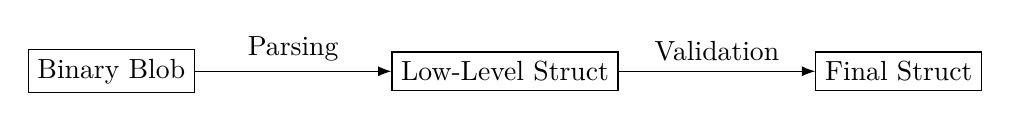
\begin{tikzpicture}
      \node[draw] (blob) at (0, 0) {Binary Blob};
      \node[draw] (ir) at (5, 0) {Low-Level Struct};
      \node[draw] (fin) at (10, 0) {Final Struct};

      \draw[-{LaTeX}] (blob) -- node[above]{Parsing} (ir);
      \draw[-{LaTeX}] (ir) -- node[above]{Validation} (fin);
    \end{tikzpicture}
    \caption{Progression from binary blob to fully parsed and validated struct.}
  \end{subfigure}

  \begin{subfigure}[b]{0.4\textwidth}
    \centering
    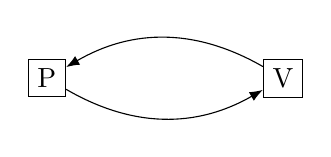
\begin{tikzpicture}
      \node[draw] (pp) at (0, 0) {P}; \node[draw] (pv) at (3, 0) {V};

      \draw[-{LaTeX}] (pp) edge[bend right] (pv); \draw[-{LaTeX}] (pv) edge[bend right] (pp);
    \end{tikzpicture}
    \caption{Protobuf parse validation loop for nested messages.}
  \end{subfigure}
  \hspace{1cm}
  \begin{subfigure}[b]{0.4\textwidth}
    \centering
    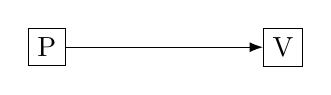
\begin{tikzpicture}
      \node[draw] (cp) at (0, 0) {P}; \node[draw] (cv) at (3, 0) {V};

      \draw[-{LaTeX}] (cp) -- (cv);
    \end{tikzpicture}
    \caption{CBOR parse validation flow. Tag 24 might require parsing again, but
    that is expected to be triggered by the host application at a later time.}
  \end{subfigure}

  \caption{Splitting the Protobuf and CDDL parse process into two steps, parsing
    and validating.}
  \label{fig:parse-validate}
\end{figure}

For Protobuf, the first step cuts the bytes into \emph{records}: a field number,
a wire type, and a raw payload. The wire type says where each payload ends, so
this needs no descriptor:
\[ \records : \mathrm{Bytes} \to \mathrm{Option}\ (\mathrm{List}\ (\id, w, \pay)). \]
The second step builds the reader's message one field at a time. The slot for
field $\id$ is $\assemble_{\dc[\id]}$ applied to $\restr{\records(\bs)}{\id}$, the
records with field number $\id$. A oneof group is handled as one unit, since a
record for one member clears the others. Records whose field number is unknown
to the reader, or whose wire type doesn't fit, are skipped. For Protobuf this
second step does more than validate: it converts numbers between types,
combines repeated records, and parses nested messages, and that is where all of
Protobuf's compatibility behaviour lives.

The compatibility relations never mention bytes. The semantic definitions of
Section~\ref{sec:framework} mention records, and only $\records$ and
$\encodes{\ty}$ mention bytes. Because each field's slot depends only on that
field's records, compatibility of whole messages follows from compatibility of
their fields.

Not every format has a first step. Avro needs the writer's schema to read
anything, and the format of Section~\ref{sec:inter-parse} cannot skip an unknown
field because its tags carry no wire type. Pollux's definition of compatibility
(Definition~\ref{def:compat}) does not depend on the split. The split is an
extra that makes field-by-field proofs possible when a format offers it.

% Local Variables:
% citar-bibliography: ("../pollux.bib")
% TeX-master: "../pollux.tex"
% TeX-command-default: "Make"
% End:


\section{Protobuf Descriptor Design}\label{sec:proto-desc}

The intermediate encoding format used a custom extensionality theorem over a
descriptor structured as a list to show that descriptors were equal. This was
required since Lean's finite maps (unlike Rocq's \texttt{gmap}) can't be placed
inside of inductive types. That's a clunky choice which was not what I wanted
when I told Aristotle ``I want extensionality on my descriptors'', but I kinda
just lived with it. Well, the full protobuf descriptors we're taking a more
principled approach that can fall back on the vast support of Mathlib.

\subsection{Protobuf Descriptors in Lean}

Instead, the full protobuf descriptors take a different approach, using a
dependently typed list internally but exposing a view of the descriptor using a
proper finite map.

\begin{minted}{lean}
inductive ScalarType where
  | double | float | int32 | int64 | uint32 | uint64
  | sint32 | sint64 | fixed32 | fixed64 | sfixed32 | sfixed64
  | bool | string | bytes

inductive Cardinality where
  | singular | optional | repeated | oneof (group : Nat)

mutual
inductive Desc      where | mk (es : List ((_ : Int) × Field))
inductive Field     where | mk (card : Cardinality) (ty : FieldType)
inductive FieldType where | scalar (s : ScalarType) | msg (d : Desc)
end
\end{minted}

Outside of Lean, we'll use this syntax for the Protobuf descriptors.

\begin{figure}[H]
  \centering
  \begin{syntax}
    \categoryFromSet[Naturals]{g, k, n}{\mathbb{N}}

    \category[Message Name]{a}
    \alternative{\mathit{id}}
    
    \category[Scalar Type]{\ty_s}
    \alternative{\double}
    \alternative{\float}
    \alternative{\ints}
    \alternative{\intl} \\
    \alternative{\uints}
    \alternative{\uintl}
    \alternative{\sints}
    \alternative{\sintl} \\
    \alternative{\fixeds}
    \alternative{\fixedl}
    \alternative{\sfixeds}
    \alternative{\sfixedl} \\
    \alternative{\bool}
    \alternative{\String}
    \alternative{\byt}

    \category[Field Type]{\ty}
    \alternative{\ty_s}
    \alternative{\nm}

    \category[Cardinality]{\card}
    \alternative{\sig}
    \alternative{\opt}
    \alternative{\rep}
    \alternative{\oneoft{g}}

    \category[Field]{\fd}
    \alternative{\field{\card}{\ty}}

    \category[Field List]{l}
    \alternative{\nil}
    \alternative{\cons{(\id, \fd)}{l}}

    \category[Reserved Set]{\res}
    \alternative{\nil}
    \alternative{\cons{(n_1, n_2)}{\res}}

    \category[Descriptor]{\dc}
    \alternative{\desc{\res}{l}}
  \end{syntax}
  \caption{Pollux syntax for Protobuf descriptors.}\label{fig:proto-desc-syn}
\end{figure}

An alternative representation of the reserved set is to insert an artificial
empty type, which all other types can be updated to but cannot be updated to any
other type itself. Then ``removing'' a field is updating a field to this empty
type $\bot$ and that would prevent that field from ever being added again,
enforcing the same mechanism as the reserved field set. However, this would
violate the totality modeling choice which closely mirrors real world Protobuf.

The use of the sigma type is important, since it let's us tie into the existing
Mathlib infrastructure for building a finite map from from the list
internals. The basic idea is that the descriptor itself is \emph{sealed}, and we
can explode one layer at a time to get a view of the descriptor through the lens
of a finite map which should enable reasoning about the descriptor using the
theory from Mathlib. This approach also is designed to respect these
requirements:

\begin{itemize}
\item \textbf{Kernel Acceptance.} Clearly we need a representation that Lean can
  handle. Under this choice, we're not storing the map directly but are still
  able to indirectly access other theorems about it.
\item \textbf{Extensionality.} The existing formulation certain variants of the
  compatibility theorems state that we recover not an equivalent value, but an
  \emph{equal} value, which \texttt{Finmap} provides.
\item \textbf{Termination Measures.} Since we have nested messages, we need to
  ensure that we can safely traverse the descriptor and recurse on the
  descriptor. Pervious formats, like the intermediate one, defined a custom
  termination metric by noting that the depth nested descriptor must be smaller
  than the containing descriptor. This works well for tree-like descriptors, but
  Protobuf does support recursive and mutually-recursive messages definitions,
  which cannot be represented by this descriptor type.
\item \textbf{Forward Compatibility.} Protobuf can represent it's own
  descriptors, but not without recursive messages. Eventually we'll have to
  support getting a descriptor into the Lean formalization, and one option is to
  model a descriptor as a value of \texttt{descriptor.proto} and then build the
  descriptor from that information. This is common in real-world protobuf
  implementations, and the sealed design should still work for this approach.
\end{itemize}

There is a well-formedness requirement on descriptors, one coming from the
internal structure of the descriptor in Lean (Definition~\ref{def:dwf}) and the
other from the Protobuf compiler (Definition~\ref{def:dlegal}).

\vspace{1em}
\begin{definition}[Descriptor Well-Formedness]\label{def:dwf}
  A descriptor $\dc$ is well-formed, denoted $\wfd{\dc}$, if all fields in
  the descriptor have a unique field number, the fields are stored in sorted
  order, and all nested descriptors are also well-formed. Additionally, the
  reserved field intervals must have $n_1 \le n_2$ and be sorted by the lower
  bound. 
\end{definition}

\vspace{1em}
\begin{definition}[Legal Descriptor]\label{def:dlegal}
  A descriptor $\dc$ is legal, denoted $\legald{\dc}$, if
  \begin{itemize}
  \item All field numbers are between 1 and $2^{29}-1$, excluding anything
    listed in the reserved set.
  \item The range 19,000 to 19,999 is included in the reserved set. This range
    is reserved by the Protobuf compiler.
  \item Pairwise, the lower bound of a reserved range must be at least two
    larger than the upper bound of the previous element. This ensures that all
    ranges which can be merged are.
  \item Message fields are always explicitly marked as optional. This conforms
    with Protobuf, which will generate a method to check message presence, and
    will allow us to initialize recursive messages.
  \item All nested descriptors within $\dc$ are also legal.
  \end{itemize}
\end{definition}

In preparation for needing to support recursive messages, Pollux uses
well-founded recursion on the size of the descriptor through the \texttt{get?}
interface. We define a function to compute the size of the descriptor below.

\vspace{1em}
\begin{definition}[Descriptor Size]\label{def:dsize}
  The size of a descriptor $\dc$ is defined as $\dsize$ below, mutually
  recursive with the size of a field $\fd$, $\fsize$.
  \begin{mathpar}

    \dsize\left(\desc{\res}{l}\right) = \begin{cases}
      0 & \text{if } l = \nil \\
      \fsize(\fd) + \dsize \left( \desc{\res}{l'} \right) & \text{if } l = \fd
                                                            \Colon l'
    \end{cases}

    \fsize(\field{\card}{\ty_s}) = 1

    \fsize(\field{\card}{\nm}) = 1 + \dsize(\Sigma(\nm))
  \end{mathpar}
\end{definition}

\vspace{1em}
\begin{definition}[Descriptor Depth]\label{def:ddepth}
\[ \ddepth(\desc{\res}{l}) = \max_{f \in l} \fdepth(\fd), \qquad
  \fdepth(\field{\card}{\ty_s}) = 0 \qquad
  \fdepth(\field{\card}{\nm}) = 1 + \ddepth \left( \Sigma(\nm) \right)
  \]
\end{definition}

Finally, the \Oneof{} cardinality needs some explanation. When looking at
the syntactic structure of a Protobuf message in a \texttt{.proto} file, the
logical way to model a \Oneof{} is likely to have a set of fields or some
other similar grouped structure. However, this isn't how Protobuf actually
models a \Oneof{} internally, and there are good reasons for Pollux to
follow their lead. 

\begin{itemize}
\item Members of a \Oneof{} share a field number namespace with the rest
  of the message. You can't define a field with identifier $\id$ in two
  \Oneof{}'s in the same message, and using the \Oneof{} cardinality
  like we have it lets the well-formedness condition handle this automatically.
\item A \Oneof{} field doesn't have a unique field number, so there is no
  key available to insert a dedicated \Oneof{} representation into the
  finite map the descriptor is modeled as.
\item A field in a \Oneof{} can't be repeated, and \Oneof{}'s can't
  be empty. Both of those requirements are structurally impossible.
\item The Protobuf underlying \Oneof{} index isn't evolution stable, since
  introducing a new \Oneof{} will shift the assigned index of everything
  later. This complicates the \Oneof{} compatibility rules, but at least
  by adopting the same representation, everything is transparent.
\item If a program called \texttt{get?} with a field in a \Oneof{}, the
  \texttt{get?} operation would need to explore the inside of the \Oneof{}
  (via a mechanism perhaps similar to \texttt{explode}) anyways.
\end{itemize}

Fortunately, checking equality on the natural number included with each
\Oneof{} cardinality provides the required information. Even with a nested
or grouped representation, the parser would still have to manually unset the
previously set field, so this representation doesn't add any unnecessary work.

\subsection{Reserved Field Numbers}

Reserved field numbers are modeled as a list of reserved ranges. These ranges
are defined using a lower and upper limit on the range, inclusive on both
sides. This is a compact way to model a set and mirrors Protobuf syntax which
allows things like \texttt{reserved 1000 to max} which would inject thousands of
elements into the reserved set. 

We've also implemented a \texttt{contains}, \texttt{containsRange}, \texttt{add}
and \textrm{remove} operation for reserved sets which provable keep the
descriptor legal (Definition~\ref{def:dlegal}). We will use set theoretic
notations for these operations since the reserved field numbers should be
semantically thought of as a set.

Some rules might state $\id \in \res_1 \cup \res_2$ or $\id \in \res_1 \cap \res_2$, which
can be de-sugared as $\id \in \res_1 \vee \id \in \res_2$ and $\id \in \res_1 \wedge \id \in
\res_2$ respectively.

At the moment, I don't believe that full support for set unions, intersections
and subset relations are needed, but these could be implemented if required.

\subsection{Sealed \& Unsealed}

While the descriptor internals use a sorted listed, the public interface should
respect a \emph{seal} by convention (lean doesn't have great mechanisms to mark
things private or opaque). The public interface is this: 

\begin{minted}{lean}
def explode (d : Desc) : Finmap (fun _ : Int => Field) :=
    d.entries.toFinmap
def get?    (d : Desc) (k : Int) : Option Field := d.explode.lookup k
\end{minted}

Where \texttt{explode} unwraps the outer-most descriptor into a Mathlib
\texttt{Finmap}, enabling proofs to use the established \texttt{Finmap}
theory. Because \texttt{Finmap} quotients over the ordering of values in the
map, the sorted-list invariant is invisible most consumers of the interface, as
long as they use the provided mechanisms when inserting into a descriptor. Some
operations do still require the well-formed predicate, such as extensional
equality, deletions and a helpful lemma which shows that if two descriptors have
the same exploded result, they must be the same descriptor.

Descriptors should be sealed. Looking at how the code for the intermediate
format is structured, descriptors are never consumed more than one layer at a
time. The serializer iterates values, not the descriptor. While looking at a
message, we check against fields as we encounter them in the value.

However, values do need to iterated over and are the basis for round-trip
proofs. Sealing the values within the parser and serializer implementation would
create more work than we desire, although the theorems will still be able to use
a variant of the explode operator if it makes more sense.

\subsection{Considerations about Ordering \& Determinism}

The Protobuf spec permits serializing and parsing fields in any order, which
seems at odd with the choice to represent the fields in a sorted list. It should
be possible to explode a layer and use the undefined iteration order of the
\texttt{Finmap} to be as generalize as possible with regards to that Protobuf
spec. However,

\begin{itemize}
\item Having the serializer return data in any order would mean that it isn't a
  pure function, which is difficult to represent in Lean. We could quotient over
  the ordering of the fields, but then we'd have to prove that every other
  function consuming the serialized output also respects the quotient type,
  which is possible but a lot of work.
\item The exact output from the parser is descriptor dependent as well as value
  dependent (recall that we can't know what value is encoded without needing to
  to a descriptor, see Section~\ref{sec:philosophy}). Having both align as an
  ordered list reduces map equivalences to syntactic list equality.
\item The Protobuf spec is also adding a requirement to the parser, that is has
  to be able to handle encodings which were produced with the fields in an
  arbitrary order, with last field wins semantics. The existing \texttt{ParseOk}
  definition used for the intermediate formalization only requires the parser to
  be correct on the output of our own serializer, not any possible encoding. It
  will need to be extended with a relational specification which allows the
  maximum possible amount of non-determinism. The soundness requirement for this
  specification would require that our serializer produces values that satisfy
  the relational spec while completeness would require that any encoding in the
  relational specification can be parsed correctly.
\end{itemize}

\subsection{New Protobuf Features}

There are three new, notable features in Protobuf that were missing from the
intermediate formate entirely.

\begin{itemize}
\item \textbf{Cardinality.} The intermediate format only had scalar values, but
  full Protobuf has repeated values. (Optional values and implicit values are
  already extremely similar, so the addition of repeated values is the most
  important). 
\item \textbf{Maps.} Maps are easy to support since we can just desugar them, as
  described in Section~\ref{sec:proto}, with a few additions for the
  restrictions on map key type and the like.
\item \textbf{Oneof.} On the wire, a \texttt{oneof} is invisible. There is no
  information included in the wire level format to describe that a field is in a
  \texttt{oneof}, it's another one of those things that we have to have a
  descriptor to know about. Individual fields still have their own field number,
  which is encoded, that comes from the name space of the whole message. The
  \texttt{oneof} really adds a parser semantic requirement about clearing the
  old field if we encounter a new encoded field in the same \texttt{oneof}, and
  overall constraint on the final message that at most one of the fields will be
  set. The \texttt{oneof} is then represented as a cardinality, with some extra
  information to determine which \texttt{oneof} in the message this field
  belongs to. This exactly mirrors how the \texttt{descriptor.proto} operates,
  and we can use natural number equality to scan the value and clear old set
  fields when needed. Since each field has exactly one cardinality, this already
  enforces that we can't have repeated fields inside a oneof and that a oneof
  can't be empty.
\end{itemize}

\subsection{Omitted Protobuf Features}

At the moment, these features are \emph{not} modeled in Pollux. Adding support
for them should be relatively straight-forward. If I've already developed
relevant rules for them, they might be included in a different color.

\textbf{Some of these features will likely be added before the work is complete.}

\begin{itemize}
\item \textbf{Reserved field numbers.} Protobuf doesn't recommend reusing field
  numbers for new fields (i.e.\ removing a field, then later adding a field with
  that same number), and that also poses a challenge to Pollux. If a field were
  added which uses and old field number, Pollux would assume that the intent is
  for the new field to be compatible with the old one. Since we expect the
  compatibility relation to be transitive, any evolving derivation of that
  message would attempt to force a connection between two fields that are
  semantically unrelated.

  Fortunately, Protobuf has a mechanism for this, reserved field numbers. You
  can set specific field numbers as reserved, then the protobuf compiler will
  ensure that you don't add a field with that number to the message in the
  future. Pollux will also enforce this, even though the Lean formalization
  doesn't track it \emph{yet}.

\item \textbf{Field names.} Every Protobuf field has a name, which is used in
  the generated code from \texttt{protoc}. These names aren't recorded at all in
  the wire format, but do impact the compatibility of a change with the rest of
  your code. At the moment, that's considered beyond the scope of Pollux.

\item \textbf{Reserved field names.} Like reserved field numbers, you can also
  reserve field names. Pollux's stance is that this is outside the domain we're
  targeting, but could be added with mechanisms similar to the reserved field
  number.

\item \textbf{Recursive Messages.} Protobuf messages (and thus descriptors) can
  be recursive. The current lean formalization enforces a tree structure on the
  descriptors. This is nice for recursion over the descriptors, but does mean we
  can't model all descriptors. The Protobuf data set does contain recursive and
  mutually recursive descriptors. It seems that these are more common in tools
  which analyze Protobuf descriptors, likely because \texttt{descriptor.proto},
  which models Protobuf descriptors as a Protobuf struct, is recursive. If we
  want to transmit protobuf descriptors into the Pollux lean formalization using
  \texttt{descriptor.proto} (a reasonable choice), we'll have to expand the
  descriptor representation to be a flat-map of named messages. See
  Table~\ref{tab:recur-summary} and Table~\ref{tab:recur-repos} for information
  about recursive messages in the Protobuf data set.

\item \textbf{Enums.} Protobuf supports enums, which shouldn't be hard to
  support in the future, but aren't present currently.

\item \textbf{Groups.} This is a Protobuf 2 feature, which still has some
  reserved encoding wire type implications. It's simply not used in Protobuf 3.

\item \textbf{Explicit Maps.} Maps can be desugared to a \texttt{repeated}
  key-value pair (See Section~\ref{sec:proto}), so no explicit representation is
  needed. Ok, this is technically \emph{not} true, since maps have additional
  requirements about the type of the key, but if we were to desugar a map to
  it's internal representation, the user would need to also desugar it to create
  something which might be problematic.

\item \textbf{Packed Scalars.} Not really a concern of the descriptor, although
  there are serious consequences of this.
\end{itemize}

\begin{table}[H]
\centering
\begin{tabular}{lcc}
    \toprule
    Metric & Count & Percentage \\
    \midrule
    Messages & 57,461 & \\
    Recursive & 831 & 1.45\% \\
    \bullet{} self-recursive & 425 & 0.74\% \\
    \bullet{} mutually-recursive & 447 & 0.78\% \\
    Contains recursion & 3,893 & 6.78\% \\
    \bottomrule
\end{tabular}
\caption[Summary of recursive protobuf messages.]{Summary statistics of
    recursive descriptor usage in the Protobuf data set. Here ``recursive''
    means directly self-recursive or in a mutually recursive cycle while
    ``contains recursion'' is any message which includes a recursive message in
    it's transitive closure. Any message which contains recursive cannot be
    represented by the current descriptor model. There are 533
    mutually-recursive cycles with the longest containing 22 messages. Note
    that there are 41 messages which are both self-recursive and
    mutually-recursive.}\label{tab:recur-summary}
\end{table}

\begin{table}[H]
\centering
\begin{tabular}{lccccc}
    \toprule
    Repository & Messages & Recursive & \% & Contains & \% \\
    \midrule
    \texttt{protocolbuffers/protobuf-go} & 605 & 110 & 18.18\% & 151 & 24.96\% \\
    \texttt{cloudwego/kitex} & 34 & 4 & 11.76\% & 7 & 20.59\% \\
    \texttt{go-kratos/kratos} & 94 & 8 & 8.51\% & 17 & 18.09\% \\
    \texttt{bufbuild/buf} & 2,922 & 210 & 7.19\% & 371 & 12.70\% \\
    \texttt{google/protobuf.dart} & 503 & 30 & 5.96\% & 59 & 11.73\% \\
    \texttt{protocolbuffers/protobuf} & 2,372 & 172 & 7.25\% & 242 & 10.20\% \\
    \texttt{googleapis/googleapis} & 49,370 & 289 & 0.59\% & 3,022 & 6.12\% \\
    \texttt{streamdal/plumber} & 286 & 2 & 0.70\% & 13 & 4.55\% \\
    \texttt{google/rejoiner} & 50 & 0 & 0.00\% & 2 & 4.00\% \\
    \texttt{googleapis/google-cloud-go} & 134 & 3 & 2.24\% & 3 & 2.24\% \\
    \texttt{uber/prototool} & 469 & 3 & 0.64\% & 6 & 1.28\% \\
    \texttt{asynkron/protactor-go} & 149 & 0 & 0.00\% & 0 & 0.00\% \\
    \texttt{colinmarc/hdfs} & 443 & 0 & 0.00\% & 0 & 0.00\% \\
    \texttt{twitchtv/twirp} & 30 & 0 & 0.00\% & 0 & 0.00\% \\
    \bottomrule
\end{tabular}
\caption[Per-repo recursive message breakdown]{A pre-repo breakdown of
    recursive message and messages which contain recursion. Notice that tools
    which work with protobuf descriptors have a higher percentage of recursive
    messages than project which just use Protobuf. The aggregate numbers in
    Table~\ref{tab:recur-summary} are dominated by
    \texttt{googleapis/googleapis} since it contains 86\% of the data set. I
    don't know what's happening with \texttt{google/rejoiner}, but it's
    possible some messages didn't compile correctly.}\label{tab:recur-repos}
\end{table}

% Local Variables:
% citar-bibliography: ("../pollux.bib")
% TeX-master: "../pollux.tex"
% TeX-command-default: "Make"
% jinx-local-words: "protobuf"
% End:


\section{Protobuf Message Design}\label{sec:proto-msg}

Mirroring the descriptors are the values, which carry actual data rather than
describe the shape of a message.

\subsection{Values in Lean}

In the Lean formalization, the structure of a value matches the structure of
descriptors across all three levels.

\begin{itemize}
\item A descriptor can be matched to a value.
\item A field can be matched to a slot.
\item A field type can be matched to a payload.
\end{itemize}

\begin{minted}{lean}
mutual
inductive Value   where | mk (es : List ((_ : Int) × Val))
inductive Slot    where | implicit (p : Payload)
                        | optional (p : Option Payload)
                        | repeated (ps : List Payload)
inductive Payload where | int (z : Int) | bool (b : Bool) | string (s : String)
                        | bytes (bs : List UInt8) | float (bits : UInt32)
                        | double (bits : UInt64) | msg (v : Value)
end
\end{minted}

Notice that just like with the descriptor, the presence wrapper sites above the
payload, and also reduces the number of constructor cases (marginally) and
creates a regular structure for \texttt{optional} and \texttt{repeated} fields
of an \texttt{option} / \texttt{list} of payloads rather than an \texttt{option}
/ \texttt{list} with a specific instance type. Actual data is represented in
Lean's native types. The \texttt{msg} payload constructor is the only major
structural difference from the descriptor, since it sits in the \texttt{Payload}
type rather than in a separate mutually inductive type. (I've eliminated some of
the difference in the formal grammar, but the distinction on the lean side is
worth noting.) However, the inductive structure \emph{does} match --- it's
under the presence modifier, but still above the leaf of the descriptor or value
--- and the descriptor's scalar type gains derivable equality by being outside the
mutually recursive block. The way that the value \texttt{Payload}'s are used,
this isn't required, they're compared against a field from the descriptor in a
way to avoid this problem. Also, doubles and floats are represented as unsigned
integers to get bit-level equality. Lean's formalization of IEEE 754 floating
point numbers is opaque and the defined equality isn't reflexive (NaN $\ne$ NaN). 

{\color{red} This might change. It's possible to pull the scalar payloads out if
needed.}

\begin{figure}[h]
  \centering
  \begin{syntax}
    \categoryFromSet[Integers]{z}{\mathbb{Z}}

    \categoryFromSet[Booleans]{b}{\mathbb{B}}

    \abstractCategory[Byte Strings]{bs}

    \abstractCategory[Strings]{\mathrm{s}}

    \categoryFromSet[32-bit Unsigned Integers]{\mathrm{u^{32}}}{[0, 2^{32})}

    \categoryFromSet[64-bit Unsigned Integers]{\mathrm{u^{64}}}{[0, 2^{64})}

    \category[Payload]{p}
    \alternative{z}
    \alternative{b}
    \alternative{\mathrm{s}}
    \alternative{bs}
    \alternative{\mathrm{u^{32}}}
    \alternative{\mathrm{u^{64}}}
    \alternative{v}

    \category[Slot]{s}
    \alternative{\impslot{p}}
    \alternative{\optslot{\none}}
    \alternative{\optslot{p}}
    \alternative{\repslot{[p_1; \dots; p_m]}}

    \category[Value List]{l}
    \alternative{\texttt{[]}}
    \alternative{(n, s) :: l}

    \category[Value]{v}
    \alternative{\msg{l}}
  \end{syntax}
  \caption{Pollux syntax for Protobuf values.}\label{fig:proto-val-syn}
\end{figure}

\subsection{Value Totality}\label{sec:value-totality}

In real-world Protobuf implementations, a value always has the exact same domain
as the descriptor which generated it. If a message has a missing field (for any
reason) and that field is marked as implicit in the descriptor, the default
value is automatically populated into the field. Pollux matches this model by
requiring that when a value is linked to a specific descriptor, the domains of
the two match exactly. This will be part of the value well-formedness
conditions. Pollux will model a missing field using either the default value for
that type, $\none$ for optional values and an empty list for
\texttt{repeated} ones, just like Protobuf.

This choice strengthens the connection between a descriptor and values under it,
since rather then being able to mix and match the two arbitrarily --- something
that no real-world Protobuf implementation allows --- the assumptions made by
Pollux closely model the data assumptions of Protobuf.

However, on the proof aspect of Pollux both directions are important and worth
concerning.
\begin{itemize}
\item \textbf{Declared implies present.} A field being declared in the
  descriptor implies that something is present here in the matching value. This
  is the \emph{no omissions requirement}.
\item \textbf{Present implies declared.} Likewise a value being present in the
  message implies that it was declared in the descriptor. This is the \emph{no
    unknown values requirement}.
\end{itemize}

Starting with the first case, this requirement arises from some trouble with the
intermediate parsing format's compatibility relation, specifically the
\textsc{M-Declare} rule, where the writer's descriptor carries a field that
isn't present in the value, and the reader gets a missing value (a
intermediate format feature not present in Protobuf, this would become the
default for the type of the field).
\[
  \infer[M-Declare]{m_1 : d_1 \msgrel m_2 : d_2 \\\\ k \not \in \dom{d_1} \\ k \not \in
    \dom{m_1} \\ f_1 \fieldrel f_2}{ m_1 : d_1[k \mapsto f_1] \msgrel m_2[k \mapsto
    \mathtt{M\_MISSING}] : d_2[k \mapsto f_2]}
\]
For that format, this rule was required since without it, the message
compatibility relation could not follow the ID compatibility relation which
characterizes what could happen to a value being serialized and parsed under the
same descriptor. The well-formedness condition on the values in the intermediate
format only constrained the value without regard for a descriptor.

Under the new totality requirement, this rule is vacuous. But why is removing it
a good thing?
\begin{enumerate}
\item This doesn't happen under the Protobuf data model, which would have
  inserted the default value when creating or parsing the value originally. This
  rule only exists since the well-formedness condition of the intermediate
  format was too weak, but becomes a case in every proof about the message
  compatibility relation that describes a case that Protobuf will never express.
\item Without totality, the intermediate format never had message equality when
  serializing and parsing under the same descriptor, and this requirement
  simplifies the proofs and theorem statements.
\end{enumerate}

In the second case, the no unknown fields requirement does two important
things:

\begin{enumerate}
\item The transformations output (Section~\ref{sec:proto-transform}) will always
  have a domain of $\dom{d_2}$ since we want to provide a value when viewed
  against $d_2$. So the keys that we lose when transforming a value $v$ are
  exactly $\dom{v} \setminus \dom{d_2}$. Having exact domain equality between
  $v$ and $d_1$ means that this is the same as $\dom{d_1} \setminus \dom{d_2}$
  and enables the descriptor level compatibility relation to characterize the
  value-level transformation. The drop rule in both the descriptor compatibility
  relation and the message one for Protobuf will be applied only at write-only
  descriptor key. Allowing unknown fields to exist in the value would break
  this, and a descriptor analysis wouldn't be able to meaningful reason about
  what happens at the value level.
\item Transforming a value from it's linked descriptor to that same descriptor
  should yield exactly the same value. Without this requirement, an unknown field
  would be dropped since Pollux doesn't track unknown fields explicitly
  (Protobuf actually does, for largely this reason, motivated by a potential
  man-in-the-middle where the sender and receiver both have a larger descriptor
  then the relay).
\end{enumerate}

At the byte level, the serializer will never emit a tag that the parser using
the same descriptor can't understand, so our prospective is that an unknown
field must come from a schema difference in the descriptors (or some
modification made to the value on the network; well outside our scope).

\subsection{Cardinality and Scalar Carriers}

The presence marker in the value layer has three constructors, while the
cardinality marker in the descriptor layer has four, with \texttt{oneof} being
the missing one. Be default in Protobuf, all \texttt{oneof} fields are treated
as \texttt{optional}, which Pollux also respects. The requirement that only one
is set is a cross-field constraint, which will live in value's legal predicate.

Additionally, while the descriptor scalar types enumerate all Protobuf type, the
value collapses several of these into a shared carrier. Specifically for all the
various integer types, the value uses a mathematical integer when the Protobuf
scalar types change in encoding and range. The legal predicate for values will
enforce the range requirement while the encoding choice is only relevant
during the serialization and parsing process, not the final values.

\subsection{Value Initialization}\label{sec:msg-init}

Since messages have to match their descriptor, it's important that we're able to
generate initial, empty messages to establish this invariant. Notice that the
\texttt{Field.init} function takes the cardinality information in addition to the
type information. This is what lets the initialization process differentiate
between the default value of a repeated field (an empty list), optional field
($\none$) and scalar field.

\begin{minted}{lean}
def Field.init : Field → Val
  | .mk .singular (.scalar s) => .implicit (ScalarType.defaultPayload s)
  | .mk .singular (.msg _)    => .optional none   -- unreachable when Legal
  | .mk .optional _           => .optional none
  | .mk .repeated _           => .repeated []
  | .mk (.oneof _) _          => .optional none

def Value.init (d : Desc) : Value := ⟨d.entries.map
    (fun e => ⟨e.1, Field.init e.2⟩)⟩

theorem Value.get?_init (d : Desc) (k : Int) :
    (Value.init d).get? k = (d.get? k).map Field.init
\end{minted}

This is one of two places where the descriptor seal is broken and (recursive) iteration over
the descriptor is performed, the other being the injection of missing fields
during parsing. 

\subsection{Value Validity} 

Descriptor validity broke down into two requirements, a Lean specific invariant
on the internal structure of our representation, and the Legal predicate that
enforces some particular requirements of the Protobuf compiler. A value being
well-formed is a bit more complex since we require that it's well-formed
\emph{against} a descriptor. The value well-formedness predicate will be used as
the output well-formedness predicate of the Protobuf serializer, meaning we'll
be able to assume that a value input to the serializer is well-formed and
use that in combination progress theorem that all well-formed values will
serialize. Validity on the value is the precondition for the top-level
round-trip theorems, and are encoded into the type of the serializer from our
serializer combinator library. The actual contents of the validity predicate are
stronger than needed to show that the serialization will always succeed, but can
be weakened to imply the needed combinator well-formedness conditions throughout the
combinator library.

\vspace{1em}
\begin{definition}[Valid Message]\label{def:vvalid}
  A message $m$ is valid against a descriptor $d$, denoted $\validv{m}{d}$ if
  both $\wfm{m}$ and $\legalv{m}{d}$. 
\end{definition}

\vspace{1em}
\begin{definition}[Message Well-Formedness]\label{def:vwf}
  A message $m$ is well-formed, denoted $\wfm{m}$, if all fields in
  the message have a unique field number, the fields are stored in sorted
  order, and all nested messages are also well-formed.
\end{definition}

\vspace{1em}
\begin{definition}[Legal Message]\label{def:vlegal}
  A message $m$ is legal with regards to descriptor $d$, denoted $\legalv{m}{d}$, if
  \begin{itemize}
  \item Totality, $\dom{m} = \dom{d}$.
  \item For all values in the message
    \begin{itemize}
    \item The presence of the field agrees with the cardinality in the
      descriptor.
    \item The type of the value agrees with the type of the field in the
      descriptor. For integer scalars, this condition also enforces the range
      bounds associated with the various Protobuf integer types (i.e.\ \ints{},
      \uintl{}, etc.) while for nested messages, that means $\validv{m'}{d'}$.
    \end{itemize}
  \item At most one key in a \texttt{oneof} group defined in the descriptor is
    set. This is the only non-pairwise requirement that a well-formed message has
    to respect.
  \end{itemize}
\end{definition}

Descriptor legality (Definition~\ref{def:dlegal}), specifically the fact that
messages have to be \texttt{optional}, is important here since it makes it
possible to initialize a recursive message, and we can assume that anytime a
message is present, it's a non-default. This means that the Pollux check for if
a value is a default can be decidable, even though descriptors and fields don't
have a decidable equality instance defined.

\vspace{1em}
\begin{lemma}
  For all descriptors $d$, $\validv{\init(d)}{d}$.
\end{lemma}

\vspace{1em}
\begin{definition}[Message Size]\label{def:vsize}
  The size of a message, $\mathrm{size}_v$, is defined below. 
  \begin{mathpar}
    \mathrm{size}_v(\lAngle l \rAngle) = 1 + \mathrm{size}_v(l)

    \mathrm{size}_v(l) =
    \begin{cases}
      0 & \text{if } l = \texttt{[]} \\
      \mathrm{size}_v(v) + \mathrm{size}_v(l') & \text{if } l = (\_, v) :: l'
    \end{cases}

    \mathrm{size}_v(v) =
    \begin{cases}
      1 + \mathrm{size}_v(p) & \text{if } v = \impslot{p} \\
      1 & \text{if } v = \optslot{\none} \\
      1 + \mathrm{size}_v(p) & \text{if } v = \optslot{p} \\
      1 + \mathrm{size}_v(p_1) + \dots + \mathrm{size}_v(p_n) & \text{if } v = \repslot{[p_1;\dots;p_n]}
    \end{cases}

    \mathrm{size}_v(p) =
    \begin{cases}
      \mathrm{size}_v(\lAngle l' \rAngle) & \text{if } p = \lAngle l'
                                              \rAngle \\
      1 & \text{otherwise}
    \end{cases}
  \end{mathpar}
\end{definition}

% Local Variables:
% citar-bibliography: ("../pollux.bib")
% TeX-master: "../pollux.tex"
% TeX-command-default: "Make"
% jinx-local-words: "protobuf"
% End:


\section{Protobuf Parser}\label{sec:proto-parse}

Following the two-step process outlined in Section~\ref{sec:philosophy}, the
Pollux Protobuf parser uses an intermediate representation to handle Protobuf.

A protobuf message on the wire is a sequence of records.

\vspace{1em}
\begin{definition}[Protobuf Record]
  A Protobuf wire record is a tuple with the field number $k$, the wire type $w$
  and the payload. The wire type will control how long the payload is.
\end{definition}

\vspace{1em}
\begin{definition}[Protobuf Record Wire Type]
  There are four Protobuf wire types represented in a record:
  \begin{itemize}
  \item \texttt{VARINT}, whose payload is an unsigned number up to $2^{64} - 1$.
  \item \texttt{I64}, whose payload is exactly 8 bytes.
  \item \texttt{I32}, whose payload is exactly 4 bytes.
  \item $\mathtt{LEN}\ \ell$, whose payload is exactly $\ell$ bytes.
  \end{itemize}
\end{definition}

% Local Variables:
% citar-bibliography: ("../pollux.bib")
% TeX-master: "../pollux.tex"
% TeX-command-default: "Make"
% jinx-local-words: "cardinality protobuf"
% End:


\section{Protobuf Transformation}\label{sec:proto-transform}

At the core of the Protobuf compatibility methodology is a transformation which
projects the view of a message under one descriptor to a related message under
another descriptor.

\subsection{Origins}

Using a function to transform the value isn't an arbitrary technical choice, nor
is it only useful to model potential descriptor changes to specific Protobuf
value. It arises naturally from the proofs of the intermediate format, and that
evolution is described here.

The first and strongest intermediate parser compatibility theorem is the
schema-correct one, Theorem~\ref{thm:inter-schema-correct}, where the relations
at play are strong enough that we can directly prove that the resulting value
from a serializer / parser round-trip under the same descriptor is equal. No
transformation is needed here.

However, the next step was to weak the compatibility antecedent to arrive at
Theorem~\ref{thm:inter-id-compat} where the descriptor is still the same but can
have no relation to the message being operated on. This is no longer possible
with our new totality conditions (Section~\ref{sec:value-totality}), but led to
the first example of a transformation function. The Intermediate ID
Compatibility relation has the \textsc{M-Drop-Unknown} rule, with no constrain
which value is dropped, and \textsc{M-Missing}, which can insert a new value
into the resulting message. Because of these rules, the induction hypothesis of
the theorem by itself is too weak to prove the whole theorem since the
compatibility relation has multiple $m_2$ related to the same $m_1$, $d_1$ and
$d_2$ so the proof must find a witness. Instead we use the transformation to
strengthen the inductive hypothesis into naming that witness and prove that
anything from the transformation will land inside the compatibility relation.

The final intermediate format theorem, Theorem~\ref{thm:inter-compat},
reinforces this. It uses the same technique with a much more complex
transformation function that actually mirrors the Protobuf transformation. Both
are a structural recursion on the reader's descriptor field list, building the
new interpretation of the value under the new descriptor using the writer's
descriptor. The Protobuf one also has the stronger justification of enforcing
the totality requirement.

\subsection{Definition}

The full definition of the transformation function is omitted, since it is not
fully defined at the time of this writing. However, it is broken down into
levels, just like the various size functions.

\begin{minted}{lean}
Value.reinterpret        (d₁ d₂ : Desc) (v : Value) : Value
Value.reinterpretEntries (d₁ : Desc) (v : Value) :
    List ((_:Int) × Field) → List ((_:Int) × Val)
Value.reinterpretAt      (d₁ : Desc) (v : Value) (k : Int) (f₂ : Field) : Val
Slot.reinterpret         (f₁ f₂ : Field) (x : Val) : Option Val
Payload.reinterpret      (t₁ t₂ : FieldType) (p : Payload) : Option Payload
\end{minted}

The \texttt{reinterpretEntries} function is basically a \texttt{map} over the
internal association list, with the required termination metric.

The \texttt{Option} in the last two function signatures is \emph{not} a
message-level optional; returning a \texttt{none} means that the value is not
carryable by the new type and the caller falls back to the default slot value,
which is exactly what the reader sees when the writer's bytes do not populate
the field at all or using the incorrect wire type.

Mathematically, the transformation where a message $m$ at descriptor $d_1$ is
transformed to $d_2$ is denoted $\coercion{d_1}{m}{d_2}$.

For each key in the reading descriptor, there are three cases.

\begin{itemize}
\item \textbf{Shared.} If both descriptors carry the payload, move it over to
  the new message, transforming it if needed.
\item \textbf{Reader only.} Inject the default value for that field.
\item \textbf{Writer only.} This is a dropped field, and since we transform the
  message by walking the \emph{reader's} fields, this case cannot arise.
\end{itemize}

The other possible cases are that there is a value in the message which isn't in
the writing descriptor or that there is a field in the writing descriptor which
isn't in the message. The totality assumption from
Section~\ref{sec:value-totality} eliminates these cases from valid messages.

The recursion here is driven by the reader's descriptor since we want to produce
a message that's total over the reader's fields. Thus the termination metric is
the size that descriptor alone, not dependent on the message being
reinterpreted.

Note that the intermediate compatibility relation didn't have a drop rule in
$\dcompat$. That was because if we encountered a dropped value, we had no way to know
if the next thing in the encoding was a scalar or a nested message and the
parsing failed. Since Protobuf encoding the wire type into the value encoding,
it's always possible to skip the unknown field without de-synchronizing the byte
stream. The Protobuf drop rule will be scoped to only be applied only when
$\dom{d_1} \not \subset \dom{d_2}$.

One final note is that the measure chain used by all the transformation layers
is only \emph{weakly} decreasing within one layer, so the measures are scaled by
4 with a per-step offset to ensure that the termination metric will actually
decrease with each application. 

\vspace{1em}
\begin{theorem}[Transformation Specification]
  For all messages $m$ and descriptors $d_1$, $d_2$, each value of the
  transformed message is equal to the result of transforming that value.
  \[ \coercion{d_1}{m}{d_2}[k] = \coercion{d_1}{m[k]}{d_2} \]
\end{theorem}

\vspace{1em}
\begin{theorem}[Transform WF]\label{thm:trans-wf}
  \[ \forall\ m, d_1, d_2.\ \wfd{d_2} \rightarrow \wfm{\coercion{d_1}{m}{d_2}} \]
\end{theorem}

\vspace{1em}
\begin{theorem}[Transform Total]\label{thm:trans-total}
  \[ \forall\ m, d_1, d_2.\ \dom{d_2} = \dom{\coercion{d_1}{m}{d_2}} \]
\end{theorem}

\vspace{1em}
\begin{theorem}[Transform Self]\label{thm:trans-self}
  \[ \forall\ m, d.\ \wfd{d} \rightarrow \validv{m}{d} \rightarrow \coercion{d}{m}{d} = m \]
\end{theorem}

\vspace{1em}
\begin{theorem}[Transform Valid]\label{thm:trans-valid}
  \[ \forall\ m, d_1, d_2.\ \validv{m}{d_1} \rightarrow \wfd{d_2} \rightarrow \mathrm{OneofPreservedAll}(d_1, d_2) \rightarrow \validv{\coercion{d_1}{m}{d_2}}{d_2} \] 
  Where
  \begin{itemize}
  \item $\mathrm{OneofPreservedAll}(d_1, d_2) = \mathrm{OneofPreserved}(d_1, d_2) \wedge
    \forall\ k, \kappa_1, d_1', \kappa_2, d_2'.\ d_1[k] = \field{\kappa_1}{d_1'} \rightarrow d_2[k] = \field{\kappa_2}{d_2'} \rightarrow
    \mathrm{OneofPreservedAll}(d_1', d_2')$
  \item $\mathrm{OneofPreserved}(d_1, d_2) = \forall\ k_1, k_2, f_1, f_1', f_2, f_2',
    g. d_1[k_1] = f_1 \rightarrow d_1[k_2] = f_2 \rightarrow d_2[k_1] = f_1' \rightarrow d_2[k_2] = f_2' \rightarrow
    f_1' = \field{\oneof{g}}{\_} \rightarrow f_2' = \field{\oneof{g}}{\_} \rightarrow \exists\ g_0. f_1 = \langle
    \oneof{g_0}, \_ \rangle \wedge f_2 = \field{\oneof{g_0}}{\_}$
  \end{itemize}
\end{theorem}

The two important theorems here are Theorem~\ref{thm:trans-self}, which states
that transforming a message against it's own transform produces the same
message, and Theorem~\ref{thm:trans-valid} which we can use to show that a
transformed value is valid.

Most of the premises for these theorems should be evident, except the
\texttt{oneof} conditions for Theorem~\ref{thm:trans-valid}. This premise is
required, and to see why consider that a writer should legitimately set two
fields outside a \texttt{oneof} and then transform to a reader where those two
fields are part of the same \texttt{oneof}. The OneofPreserved function states
that any two reader keys sharing a \texttt{oneof} group were already in a group
together in the writer. Note that this is vacuous if either key is reader-only,
so adding a new field to an existing \texttt{oneof} is acceptable, while moving
an existing field into an existing \texttt{oneof} isn't. This is part of the
Protobuf best practices guide~\cite{LanguageGuideProto}, represented as proof
obligation here. The direction is also important, since it does allow us to
split a \texttt{oneof} into multiple \texttt{oneof} groups without
issue. Additionally, the recursive version is required to prevent the example
case from appearing in a nested message.

Now, it is possible to move an existing field into an existing \texttt{oneof} in
a Protobuf descriptor. In that case, you'd need to be sure that the value didn't
set multiple fields in a \texttt{oneof} of the reader (we'll know in advance
that it can't have multiple fields set in a writer's \texttt{oneof}). Then you
might be able to weaken the $\mathrm{OneofPreservedAll}(d_1, d_2)$ to 
\[ \forall\ k_1, k_2, g.\ d_2[k_1] = \langle \oneof{g}, \_ \rangle \rightarrow d_2[k_2] = \langle \oneof{g}, \_ \rangle \to
  m[k_1] = \none \vee m[k_2] = \none \]
Which is wouldn't be true for all messages under $d_1$, but might be provable
as a weakened version of Theorem~\ref{thm:trans-valid} for some systems.

{\color{red} This is another place were the functional transformation breaks
  down. In the lean serializer, everything is serialized in sorted field key
  order, so the last writer wins rule (Section~\ref{sec:last-writer-wins}) would
  be deterministic. However, since a real serializer could serialize in an
  arbitrary order, this is actually a non-deterministic operation. The
  relational encodes definition would allow this and further complicate the
  non-canonical Protobuf encoding.}

\subsection{Faithfulness Theorem}

The Protobuf compatibility framework might drop the message compatibility
relation in favor of only having the transformation. In that case, we'd end up
needing to argue that the transformation is total over all possible messages
being converted between two descriptors, i.e. $\coercion{d_1}{m}{d_2}$ produces
some $m'$ for all $\validv{m}{d_2}$.

The current transformation function is \emph{always total} by falling back to
injecting field type defaults, so in the context of Protobuf, we want to show
that we can produce a total transformation without needing this behavior outside
of injecting the new values for new fields (since any other place were a default
value is injected would imply that something failed to reinterpret). Note that
this theorem can't be solely stated about the output of
$\coercion{d_1}{m}{d_2}$ since the output can't differentiate between the
default value naturally occurring and being injected due to a problematic
update.

\begin{minted}{lean}
theorem Slot.reinterpret_isSome {f₁ f₂ : Field} {x : Slot}
    (h : f₁ ∝ f₂) (hm : Slot.Matches x f₁) :
    (Slot.reinterpret f₁ f₂ x).isSome
\end{minted}

Including \texttt{Slot.Matches} is important since incompatible cardinalities or
types between the slot and the original descriptor would invoke the default
value fallback anyways. This could be built into a faithfulness theorem.

\vspace{1em}
\begin{theorem}[Faithfulness]\label{thm:faith}
  For two compatible descriptors, $d_1 \dcompat d_2$ and a valid value $m$ under
  $d_1$, $\validv{m}{d_1}$ such that for all keys $k$, $d_1[k] = f_1$ and $d_2[k] =
  f_2$ there must exist a value $x$ and $y$ such that
  \begin{itemize}
  \item $m[k] = x$
  \item $\coercion{f_1}{m}{f_2} = y$
  \item $\coercion{d_1}{m}{d_2}[k] = y$
  \end{itemize}
\end{theorem}

Which basically characterizes the reinterpretation process as point-wise over the
message.

\begin{minted}{lean}
theorem Value.get?_reinterpret_of_compat {d₁ d₂ : Desc} {v : Value} {k f₁ f₂}
    (h : d₁ ≪ d₂) (hv : Value.Valid d₁ v)
    (h₁ : d₁.get? k = some f₁) (h₂ : d₂.get? k = some f₂) :
    ∃ x y, v.get? k = some x ∧ Slot.reinterpret f₁ f₂ x = some y ∧
      (Value.reinterpret d₁ d₂ v).get? k = some y
\end{minted}

Some corollaries from this include the fact that repeated slots don't drop
values. If the scalar transformation is only the identity function, which is
presently the case, we also have that
$\coercion{d_2}{\coercion{d_1}{m}{d_2}}{d_{2}} = m$ since the newly injected
fields are simply dropped in the backwards directly. This means that no data is
lost, but the statement is too strong to handle scalar conversion and in
particular integer width changes which might truncate values.

\vspace{1em}
\begin{theorem}[Point-wise Field Compatibility]\label{thm:pointwise-compat}
  \[ \wfd{d_1} \rightarrow \forall\ k \in \dom{d_1} \cap \dom{d_2}. d_1[k] \fieldrel d_2[k] \] 
\end{theorem}

Combined with Theorem~\ref{thm:faith}, Theorem~\ref{thm:pointwise-compat} states
that the descriptor relation $\dcompat$ is a maximal relation or equivalently
the weakest precondition for lossless data transmission. Again, this will be
complicated by adding integer truncation. Once that feature is added, this
concept is split into \emph{carriage}, which thinks about data being present,
and \emph{lossless-ness} that the transformed view of the data is unique.

% Local Variables:
% citar-bibliography: ("../pollux.bib")
% TeX-master: "../pollux.tex"
% TeX-command-default: "Make"
% jinx-local-words: "protobuf"
% End:


\section{Protobuf Compatibility Relations}~\label{sec:proto-relations}

Compatibility between protobuf entities is defined with a series of
relations. The first and most self-contained relation is the value relation,
which relates two values at the specification level if serializing just a value
(such as a variable width integer) and then parsing it to a different protobuf
type would lead to a different value. After that is the protobuf type relation,
which relates two protobuf types if any value of the first type is related to
some value of the second type in the value relation. Since protobuf field and
message definitions will not have concrete values associated with them, the type
relation can be used in place of the value relation to make safe type
changes. Finally, the message relation connects compatible messages such that
all instances of the original message can be parsed into instances of the updated
message.

Below is a list of all meta-variables used across all relations, and even across
encoding formats. When multiple of these variables are needed, you will see
variants with subscript numbers or apostrophes.

\begin{align*}
  \m &: \text{message} & v &: \text{value} \\
  \id &: \text{field number} & \ty &: \text{type} \\
  \res &: \text{Reserved field set} & \mathtt{n},\ \mathtt{m} &: \text{bit width} \\
  \fd &: \text{Field} & \card &: \text{cardinality}
\end{align*}

Below is a list of the relations about to be defined, along with an English
explanation of how to read them.

\begin{align*}
  \valrel &: \text{Value relation} & v_1 : \ty_1 \valrel v_2 : \ty_2 &\rightarrow \text{``}v_1 : \ty_1 \text{ becomes } v_2 :
                                           \ty_2 \text{''} \\
  \typrel &: \text{Type relation} & \ty_1 \typrel \ty_2 &\rightarrow \text{``}\ty_1\text{ is type-compatible with }
                                          \ty_2\text{''} \\
  \dcompat &: \text{Descriptor relation} & \dc_1 \dcompat \dc_2 &\rightarrow \text{``}\dc_1 \text{ is compatible with } \dc_2\text{''}
\end{align*}


\subsection{Value Relation}~\label{sec:val-rel}

The value relation is the base level of the compatibility relations, relating
just two individual values. Protobuf values are modeled here as a specification
level type in Lean associated with a protobuf type as listed in
Table~\ref{tab:val-spec}. Finally, while protobuf decorators are technically
part of the field level specification, they have been incorporated into the type
information to allow the specification type into include \texttt{option} or
\texttt{list} Lean types.

\begin{table}[H]
	\centering
	\begin{tabular}{cl}
      \toprule
      Specification Type & Protobuf Type \\
      \midrule
      $\mathbb{Z}$ & $\ints$, $\uints$, $\sints$,
            $\intl$, $\uintl$, $\sintl$ \\
      $\mathbb{B}$ & $\bool$    \\
      $\String$ & $\String$    \\
      \texttt{list w8}  & $\byt$    \\
      Bit Pattern & $\float$, $\double$ \\
      \bottomrule
	\end{tabular}

	\vspace{4mm}
	\caption[]{Description of the Lean type corresponding to each protobuf
      type. Floating point numbers are included in the model, but don't have a
      meaningful compatibility story, so they don't appear in the relations
      defined below.}\label{tab:val-spec}
\end{table}

While it might be tempting to have a roundtrip theorem where the output of the
serializer is passed directly to the parser, this would require a canonical
encoding, which Protobuf doesn't have. Instead we make use of a relational
encoding specification, where $\encodes{\ty}(v, \bs)$ means that $v$ can be encoded
as bytes $\bs$ under type $\ty$.

\vspace{1em}
\begin{definition}[Value Relation]
  A protobuf value at the specification level $v_1$ with protobuf type $\ty_1$ is
  related to another value $v_2$ at type $\ty_2$, denoted $v_1 : \ty_1 \valrel v_2 : \ty_2$
  if $\forall\ \bs, \encodes{\ty_1}(v_1, \bs) \rightarrow parse_{\ty_2}(\bs) = v_2$.
\end{definition}

\subsubsection{Basic Rules}

The value relation is reflexive and transitive, however a direct transitivity
rules isn't included in the relation. To understand why, first consult the
integer rules in Section~\ref{sec:proto-compat-ints} and consider what happens
when an integer is cast to a smaller byte width. Specifically, consider $2^{40}$
as a \uintl. Casting this value to a \uints{} can be done with
the \textsc{Uint-Chg-W} rule, resulting in
$2^{40} : \uintl \valrel 0 : \uints$, which describes changing
the field perfectly. However, we can then promote this field back to
\uintl{} with another application of \textsc{Uint-Chg-W}, getting
$0 : \uints \valrel 0 : \uintl$. Having a transitive rule
would result in $2^{40} : \uintl \valrel 0 : \uintl$ but
clearly parsing a serialization of $2^{40}$ as a \uintl{} when it was
serialized as a \uintl{} should recover the original value!

\begin{mathpar}
  \infer[Refl]{ }{v:\ty \valrel v:\ty}
\end{mathpar}

\subsubsection{String \& Byte Rules}

It is possible to convert been the \String{} and \byt{} types,
although the host program may have to deal with control character bytes being
present in the resulting string. Technically the Protobuf specification requires
that all strings are encoded in UTF-8, so we can optionally add that requirement
to converting from \byt{} to \String.

\begin{mathpar}
  \infer[Str-Byte]{ }{v: \String \valrel v: \byt}

  \infer[Byte-Str]{ {\color{red} v \text{ is valid UTF-8}} }{v: \byt \valrel v: \String}
\end{mathpar}

\subsubsection{Varint Scalar Rules}\label{sec:proto-compat-ints}

Every integer type and several non-integer protobuf types are encoded using the
variable-width integer encoding described in Section~\ref{sec:proto-vint}. To
compactly represent 30 rules, we'll observe that all the varint-encoded values
are transmitted over the wire in the range $\payload$. We can factor each
rule as using the writer's type to convert it to the wire value, then the
reader's type to convert it to the new parsed value.

As a shorthand, statements like \uintn{n} represent a variable length integer
encoding into $\width$ bits. In order to result in valid protobuf types,
$\width \in \{32, 64\}$.

It is also worth noting that the expression $v : \ty$ actually refers to a value
of type $\denote{\ty}$ with a label of the type. All of the integer
types have $\denote{\cdot} = \mathbb{Z}$, as shown in Table~\ref{tab:val-spec},
which allows for the free conversion between integer types. Finally, $\%$ refers
to modulus using floored division, so $-1 \fmod 2 = 1$ and the rules are
written with truncated integer division.

Let $\vints = \left\{ \uintn{n}, \intn{n}, \sintn{n}, \bool \right\}$ represent
the protobuf types encoded on the wire as a variable-width integer. For each
$\ty \in \vints$, let
\begin{align*}
  \encop{\ty} &: \denote{\ty} \rightarrow \payload \\
  \decop{\ty} &: \payload \rightarrow \denote{\ty}
\end{align*}
be functions that convert from a $\ty$-typed writer to the payload number and
the value recovered by a $\ty$-typed reader respectively.
\[
  \infer[Varint]{ \ty_1, \ty_2 \in \vints \\ v_2 =
    \dec{\ty_2}{\enc{\ty_1}{v_1}}}{v_1 : \ty_1 \valrel v_2 : \ty_2}
\]

The table below gives the decoding and encoding functions for each type, and
makes use of the following definitions.

\begin{table}[H]
  \centering
  \begin{tabular}{l c c}
    \toprule
    $\ty$ & $\enc{\ty}{v}$ & $\dec{\ty}{x}$ \\
    \midrule
    \uintn{n} & $v$ & $x \fmod 2^{\width}$ \\
    \intn{n} & $v \fmod 2^{\width}$ & $((x + 2^{\width-1}) \fmod 2^{\width}) - 2^{\width-1}$ \\
    \sintn{n} & $\zz{v}$ & $\unzz{x \fmod 2^{\width}}$ \\
    \bool & $\ind{v}$ & $x \ne 0$ \\
    \bottomrule
  \end{tabular}
  \caption[Encoding and decoding rules for Varint conversions.]{Payload written
    and value recovered for each varint-encoded type. Here $\%$ is always the
    non-negative floored modulus; no truncated division occurs. The
    $\encop{\intn{n}}$ row is the ten-byte sign extension: protobuf writes every
    negative $\intn{n}$ as its two's complement at 64 bits, which is exactly
    $v \fmod 2^{64}$.
  }
  \label{tab:varint-conversion}
\end{table}

Which uses these definitions for converting to and from the zig-zag encoding
(See Section~\ref{sec:proto}).
\begin{align*}
  \zz{v} &= \left\{
    \begin{array}{l@{\quad:\quad}l}
      2v & v \ge 0 \\
      -2v - 1 & v < 0
    \end{array}\right. \\
  \unzz{x} &= \left\{
    \begin{array}{l@{\quad:\quad}l}
      x / 2 & x \text{ even} \\
      -(x + 1) / 2 & x \text{ odd.}
    \end{array}\right.
\end{align*}

Using these functions, we can still derive and simplify every rule for
converting between varint scalars.

\begin{table}[H]
  \centering
  \begin{tabular}{lcccc}
    \toprule
    \multirow{2}{*}{writer $v_1 : \ty_1$} & \multicolumn{4}{c}{reader $\ty_2$} \\
    & \uintn{m} & \intn{m} & \sintn{m} & \bool{} \\
    \midrule
    \uintn{n} & $v_1 \fmod 2^m$      & $\tosigned{m}{v_1}$      & $\unzz{v_1 \fmod 2^m}$      & $v_1 \ne 0$ \\
    \intn{n}  & $v_1 \fmod 2^m$      & $\tosigned{m}{v_1}$      & $\unzz{v_1 \fmod 2^m}$      & $v_1 \ne 0$ \\
    \sintn{n} & $\zz{v_1} \fmod 2^m$ & $\tosigned{m}{\zz{v_1}}$ & $\unzz{\zz{v_1} \fmod 2^m}$ & $v_1 \ne 0$ \\
    \bool{}   & $\ind{v_1}$   & $\ind{v_1}$    & $-\ind{v_1}$         & $v_1$ \\
    \bottomrule
  \end{tabular}
  \caption{The transform induced by \textsc{Varint} on every pair of
    varint-encoded types, writing
    $\tosigned{m}{x} = \left((x + 2^{m-1}) \fmod 2^m\right) - 2^{m-1}$ for the
    reader's signed truncation.  Widths $\width$ and $m$ are independent, so this
    covers all thirty non-identity conversions.}\label{tab:varint-derived}
\end{table}

\subsubsection{Message Rules}

Definitions for the structure of a messages are given in
Section~\ref{sec:msg-rel}. The values are represented as a mapping from the id
number of each field to the value and type of that field. 

\begin{mathpar}
  \infer[Msg]{\desc{\res_1}{f_1} \msgrel \desc{\res_2}{f_2} \\ \forall\;\id \in \dom{v_2}.\;\left( f_1(\id) =
      (\card, \ty_1) \wedge v_1(\id) \valrel v_2(\id) \right) \vee v_2(\id) = default\left(\mathtt{snd}\ f_2(\id)\right)}
  {v_1 : \mathtt{MSG}\ \desc{\res_1}{f_1} \valrel v_2 : \mathtt{MSG}\ \desc{\res_2}{f_2} }
\end{mathpar}

The first rule is complex. It stands that a message with some reserved fields
and field definitions can be interpreted as a message with a different set of
reserved fields and field definitions if the two descriptors are compatible and
if for all fields in the resulting value, either (1) it has a compatible value
(2) it has the default value.

\subsubsection{Decorator Rules}

Since the specification type can include \texttt{option}'s and
\texttt{repeated}'s, rules for handling these must also be present in the value
relation. These rules are grouped into introduction rules, which take implicit
values and make them optional or repeated, pass through rules which enable the
above rules to operate on these modified types.

Generally speaking, we can introduce, eliminate {\color{red} (It's clear what
  happens when we eliminate a non-packed \texttt{repeated} field; the last
  writer wins. What happens when we eliminate a packed field? We'll end up
  skipping the field as unknown. This difference is actually why we can't have a
  \textsc{Rep-Elim} rule since we can't implement the elimination as a function
  without more knowledge.)} or change the
underlying type of each decorator. Implicit fields require no special
consideration.

\begin{mathpar}
  \infer[Rep-Pass]{v_1:\ty_1 \valrel v_1':\ty_2 \\ \cdots \\ v_n:\ty_1 \valrel v_n':\ty_2}{[v_1; \dots;
    v_n]: \rept{\ty_1} \valrel [v_1'; \dots; v_n']: \rept{\ty_2}}

  \infer[Opt-Some-Pass]{v_1:\ty_1 \valrel v_2:\ty_2}{(\some{v_1}): \optt{\ty_1} \valrel
    (\some{v_2}): \optt{\ty_2}}

  \infer[Opt-None-Pass]{ }{\none: \optt{\ty_1} \valrel \none: \optt{\ty_2}}
  
  \infer[Opt-Intro]{ }{v:\ty \valrel (\some{v}): \optt{\ty}}

  \infer[Rep-Intro]{ }{v:\ty \valrel [v]: \rept{\ty}}

  \infer[Missing-Imp]{\ty_1 \typrel \ty_2}{\none: \ty_1 \valrel default(\ty_2):\ty_2}
\end{mathpar}

\subsection{Type Relation}~\label{sec:typ-rel}

This relation relates types which can be converted via the value
relation. Recall that this relation is needed to reason about descriptor-only
compatibility, which doesn't have any concrete values associated with it.

\begin{definition}[Type Relation]
  The type relation relates two protobuf type $\ty_1$ and $\ty_2$, denoted $\ty_1 \typrel
  \ty_2$ if for all $v_1:\ty_1$ there exists a $v_2:\ty_2$ such that $v_1:\ty_1 \valrel v_2:\ty_2$.
\end{definition}

These rules compress many of the rules in the previous section into one rule,
stating that types are compatible with each other.

\subsubsection{Base Type Rules}

\begin{mathpar}
  \infer[Str-Byt-T]{ }{\String \typrel \byt}

  \infer[Byt-Str-T]{ }{\byt \typrel \String}

  \infer[Int-Int-T]{\ty_1, \ty_2 \in \left\{{
        \begin{array}{c}
          \ints, \intl, \uints, \uintl \\
          \sints, \sintl, \bool
        \end{array}
      }\right\}}{\ty_1 \typrel \ty_2}
\end{mathpar}

It's worth pointing out that converting to and from \sintn{n} is tricky, since
the values can change in ways that most programmers aren't expecting, although
that integer type is perfectly compatible with Protobuf's wire format. Practical
usage of Pollux as a rule should probably remove \sints{} and \sintl{} from the
\textsc{Int-Int-T} rule. The inclusion of those integer types here also diverges
from Protobuf's official compatibility guide \cite{LanguageGuideProto}.

\subsubsection{Message Rules}

\begin{mathpar}
  \infer[Msg-T]{m_1 \msgrel m_2}{\mathtt{MSG}\ m_1 \typrel \mathtt{MSG}\ m_2}
\end{mathpar}

\subsubsection{Decorator Rules}

Since the type relation is designed for checking for safe type changes, it also
need to ensure that decorator restrictions like moving from a repeated field to
a singleton one aren't violated.

\begin{mathpar}
  \infer[Opt-Add-T]{ }{\ty \fieldrel \optt{\ty}}

  \infer[Opt-Rm-T]{ }{\optt{\ty} \fieldrel \ty}

  \infer[Opt-T]{\ty_1 \typrel \ty_2}{\optt{\ty_1} \fieldrel \optt{\ty_2}}

  \infer[Rep-Add-T]{ }{\ty \fieldrel \rept{\ty}}

  \infer[Rep-T]{\ty_1 \typrel \ty_2}{\rept{\ty_1} \fieldrel \rept{\ty_2}}
\end{mathpar}

\subsection{Message Relation}~\label{sec:msg-rel}

The descriptor compatibility relation $\dcompat$ is defined as below, but first
it is important to discuss the structure of fields and messages.

A message value is a tuple containing a set of reserved field numbers and names,
then a map from an identifier to a tuple with the name of the field and the type
of the field. The identifier is either a tag for a single field, or a set of
integers which is used for a \Oneof, where multiple fields must be
mutually exclusively set.

Enums will be modeled as a set of integers, likewise ignoring the name given to
each element to favor the integer which is used in the encoding. The enum
relation is defined using $\enumrel$ to differentiate it from the message
relation.

\subsubsection{Basic Rules}

A compatibility relation is both reflexive and transitive, although it is
neither symmetric nor anti-symmetric.  

\begin{mathpar}
   \infer[Refl-M]{ }{m \msgrel m}

   \infer[Refl-E]{ }{e \enumrel e}

   \infer[Trans-M]{m_1 \msgrel m_2 \\ m_2 \msgrel m_3}{m_1 \msgrel m_3}

   \infer[Trans-E]{e_1 \enumrel e_2 \\ e_2 \enumrel e_3}{e_1 \enumrel e_3}
\end{mathpar}

\subsubsection{Field Update Rules}

For the moment, names are recorded the protobuf field descriptors for accuracy
and to allow the relations to expand in the future. However, since names are not
recorded in the encoded message, they are currently allowed to freely change.

{\color{red} I seem to remember Tej saying that we \emph{should} have the name
  information available somewhere in the descriptor. I need to check my notes
  about that.}

Generally speaking, we can change the type of a field, add a new field or update
a field in a map.

\begin{mathpar}
  \infer[Field-Type]{f(id) = \ty_1 \\ \ty_1 \typrel \ty_2}{\desc{\res}{f} \msgrel \desc{\res}{f[id \mapsto \ty_2]}}

  \infer[Field-Add]{id \not \in \dom{f}}{\desc{\res}{f} \msgrel \desc{\res}{f[id \mapsto \ty]}}

  % TODO: May need restrictions about maps in maps...
  \infer[Map-Type-F]{f(id) = (\map{\ty_1}{\impt{\ty_2})} \\ \ty_1 \typrel \ty_1' \\ \ty_2
    \fieldrel \impt{\ty_2'} \\ \ty_1 \ne \byt} {\desc{\res}{f} \msgrel \desc{\res}{f[id \mapsto
      (\map{\ty_1'}{\impt{\ty_2'}})]}}
\end{mathpar}

Messages are similar to records in Lean or other functional languages and
message compatibility can take the same two routes that record subtyping can:
width compatibility and depth compatibility. In width compatibility updates, new
fields are added to the message, making the updated version a strict superset of
the original message. In depth compatibility updates, the number of fields
remains the same, but other attributes of the field are updated compatible ways.

\subsubsection{Oneof Rules}

The \Oneof{} rules are a bit complicated because a \Oneof{}
struggles against the notion that the field relations only connects one field to
one field by encapsulating several fields into a singular field.

% FIXME: Oneof fields don't cleanly fit into the map abstractions since there is
% no clear choice of key.

\begin{mathpar}
  \infer[Oneof-Intro-Field]{\card \in \{\imp, \optt\} \\ f(id) = \field{\card}{\ty}}
  {\desc{\res}{f} \msgrel \desc{\res}{f[\{id\} \mapsto \oneof{id \mapsto \field{\card}{\ty}}]}}

  % May need some statement about f_{n+1} not already being in the message?
  % You can introduce a new field, but not move an existing one.
  \infer[Oneof-Add-F]{\card \in \{\imp, \optt\} \\ id_n \not \in
    id_s \\ f(id_s) = m \\ id_n \not \in  \dom{m} \\ \ty \not= \mathtt{MAP}}
  {\desc{\res}{f} \msgrel \desc{\res}{f[id_s \cup \{id_n\} \mapsto (m[id_n \mapsto \field{\card}{\ty}])]}}

  % This rule should just be a combination of the above two rules...
  \infer[Oneof-Intro-New]{\dom{ f } \cap \dom{ f_o } = \emptyset
    \\ \rep \not \in dec(f_o) \\ \forall\;id_n \in \dom{f_o}.\
    \texttt{snd}\ f_o(id_n) \ne \mathtt{MAP}}{\desc{\res}{f} \msgrel \desc{\res}{f[\dom{f_o}
      \mapsto f_o]}}

  \infer[Oneof-Elim]{f(id_n) = m \\ id \in id_n }
  {\desc{\res}{f} \msgrel \desc{\res}{f[id_n \setminus id \mapsto m \setminus id]}}

  % I'm not sure about the premise of this rule, but it seems better than having
  % to making another version of all the other rules. This is the first instance
  % where having a field relation would be very helpful.
  \infer[Oneof-Field-Update]{f_o(id') = \ty \\ \ty \typrel \ty'}
  {\desc{\res}{f[id \mapsto f_o]} \msgrel \desc{\res}{f[id \mapsto ( f_o[id' \mapsto \ty'] )]}}
\end{mathpar}

\subsubsection{Enum Rules}

The enum rules are similar to the message rules at least in the sense that enums
can be updated to have new fields without issue. However, when considering
removing fields from an enum definition, it is important to know if the enum is
treated as open or closed~\cite{EnumBehavior}. By default, \texttt{proto3}
treats all enums as open, so it should be possible to write a rule allowing for
the deletion of an enum field. This naturally aligns with how \texttt{go}
handles enums, since it doesn't support closed enums. Since protobuf enums don't
contain extra information, no depth rules is allowed.

\begin{mathpar}
  \infer[Enum-Width]{vals(e_1) \subset vals(e_2)}{e_1 \enumrel e_2}
\end{mathpar}

\subsubsection{Reserved Field Rules}

\begin{mathpar}
  \infer[Reserved-Add]{\res \subset \res'}{\desc{\res}{f} \msgrel \desc{\res'}{f}}

  {\color{red}
    \infer[Reserved-Rm]{\res \supset \res'}{\desc{\res}{f} \msgrel \desc{\res'}{f}}
  }
\end{mathpar}

\subsubsection{Valid Descriptors}

\begin{definition}[Valid Protobuf Descriptors]
  A protobuf message descriptor is \emph{valid}, denoted $v(\dc)$ if
  $\desc{\emptyset}{\emptyset} \msgrel \desc{\res}{f}$.
\end{definition}

\subsubsection{Compatibility Theorem}

The main field-level compatibility theorem is stated below.

\vspace{1em}
\begin{theorem}[Protobuf Compatibility]
  If $\dc_1 \dcompat \dc_2$ and $\dc_2$ is well-formed, then for all binary strings
  $\bs$ such that $\mathtt{parse}_{\dc_1}\ \bs = \some{\m_1}$,
  $\mathtt{parse}_{\dc_2}\ \bs = \some{\m_2}$ and $\m_1 \msgrel \m_2$
\end{theorem}

% Local Variables:
% citar-bibliography: ("../pollux.bib")
% TeX-master: "../pollux.tex"
% TeX-command-default: "Make"
% jinx-local-words: "protobuf"
% End:


\section{A Type-Theoretic Approach}\label{sec:type-theory}

If we view descriptors as record types (which they clearly are), we can borrow
concepts from Programming Languages theory. Specifically, taking the view that
serializing then parsing under a different descriptor is a coercion and can be
modeled as such, we can draw some literature on subtyping as
coercions~\cite{breazu-tannenInheritanceImplicitCoercion1991,brandtCoinductiveAxiomatizationRecursive1998}. 

\subsection{Compatibility as Coercion}

Pollux's goal is to be able to look at a pair of data descriptors and
characterize what happens to values under the first descriptor when parsed under
the updated one. Our derivations, of the form $\judg{\varnothing}{\dc_1 \dcompat \dc_2}$
provide more than a certificate of compatibility between the descriptors: read
rule by rule, it is a program $\co : \denote{\dc_1} \rightarrow \denote{\dc_2}$, a coercion the
reader applies to the writer's message.

\vspace{1em}
\begin{definition}[Well-behaved Transformation]\label{def:well-behaved}
  A coercion $\co : \denote{\dc_1} \to \denote{\dc_2}$ is \emph{well-behaved} when,
  for all $\validv{\m}{\dc_1}$ and all $\bs$ with $\encodes{\dc_1}(\m, \bs)$,
  \[ \mathrm{parse}_{\dc_2}(\bs) = \some{(\co(\m), U)} \quad\text{with}\quad
    U \subseteq \dom{\dc_1} \setminus \dom{\dc_2}. \]
\end{definition}

\vspace{1em}
\begin{definition}[Compatibility]\label{def:compat}
  Two descriptors $\dc_1$ and $\dc_2$ are compatible if there exists a well-behaved
  transformation between them. 
\end{definition}

Here $U$ is the set of fields skipped during parsing (i.e.\ writer-only fields or
fields with mismatched wire types). The second condition that
$U \subseteq \dom{\dc_1} \setminus \dom{\dc_2}$ is essential to this definition. Wire-soundness,
that the message parses, would admit something like $\ints \dcompat \String$ when the
reader skips the mistyped record and injects the default $\String$ value. This
condition rules out the trivial transformation which always injects the default
values for all fields.

There are two conditions part of Definition~\ref{def:well-behaved}, wire
soundness and faithfulness. Wire soundness states that a valid encoding of a
message under $\dc_1$ will parse to the coerced version under $\dc_2$. Faithfulness
states that there are no skipped fields during parsing.  An immediate
consequence of this definition is that coherence is free. Wire soundness pins
$f$ down on every valid message that has at least one encoding. So if
$\encodes{\dc_1}$ is total on valid messages (i.e. a serializer exists), any two
derivations of the same judgment yield coercions that agree on valid messages.

\subsubsection{Pollux Judgements}

A Pollux judgment has the form $\judg{\Gamma}{\dc_1 \dcompat \dc_2 \coerce \co}$ where
\begin{itemize}
\item $\Sigma$ is a symbol table, mapping names of descriptors to descriptor
  values. Representing this as a table allows us to store (mutually) recursive
  descriptors in finite syntax and mirrors Protobuf's own
  \texttt{FileDescriptorSet} construct.
\item $\Gamma$ is the assumption context, which stores pairs of descriptor names
  which are assumed to be compatible with each other. It maps pairs of
  descriptor names to \emph{assumption variables} which will hold the coercion
  between those descriptors in the completed derivation. An alternative
  formulation would be so that $\Gamma$ maps a pair of descriptors to a value of type
  $x : \denote{\Sigma(\nm_1)} \rightarrow \denote{\Sigma(\nm_2)}$ 
\item $\co$ is a function $\co : \denote{\Sigma(\dc_1)} \rightarrow \denote{\Sigma(\dc_2)}$, the coercion
  built by the derivation.
\end{itemize}

This is actually a stratified definition, yielding slightly different coercions
for each type of object:
\begin{align*}
  &\judg{\Gamma}{\dc_1 \dcompat \dc_2 \coerce \co}
  && \co : \denote{\dc_1} \to \denote{\dc_2} \text{ (message bodies)} \\
  &\judg{\Gamma}{\fd_1 \fieldrel \fd_2 \coerce \co}
  && \co : \denote{\fd_1} \to \denote{\fd_2} \text{ (fields: cardinality and type)} \\
  &\judg{\Gamma}{\ty_1 \typrel \ty_2 \coerce \co}
  && \co : \denote{\ty_1} \to \denote{\ty_2} \text{ (payloads)}
\end{align*}

\subsubsection{Names \& Recursion}

\begin{mathpar}
  \infer[N-Assum]
    { \Gamma((\nm_1, \nm_2)) \mapsto x }
    { \judg{\Gamma}{\nm_1 \dcompat \nm_2 \coerce x} }

  \infer[N-Unfold]
    { (\nm_1, \nm_2) \notin \dom{\Gamma} \\
      \judg{\Gamma, (\nm_1, \nm_2) \mapsto x}{\Sigma(\nm_1) \dcompat \Sigma(\nm_2) \coerce \co} }
    { \judg{\Gamma}{\nm_1 \dcompat \nm_2 \coerce \mathsf{fix}\ x.\ \co} }
\end{mathpar}

The fix-point operator $\mathsf{fix}$ is well founded on the writer's value
since the $x$ is only ever applied under the \textsc{F-Msg} rule, which means
it's applied to a nested message of strictly smaller depth.

\subsubsection{Descriptors}

\begin{mathpar}
  \infer[D-Update]
  { \forall \id \in \dom{\dc_1} \cap \dom{\dc_2}.\ \judg{\Gamma}{\dc_1[\id] \fieldrel \dc_2[\id] \coerce \co_{\id}} \\
    \mathrm{OneofPreserved}(\dc_1, \dc_2) }
  {
    \judg{\Gamma}{\dc_1 \dcompat \dc_2 \coerce \lambda \m.\
      \forall\ \id \in \dc_2.
      {\begin{cases}
        \id \mapsto \co_{\id}(\m[\id]) & \id \in \dom {\dc_1} \cap \dom{\dc_2} \\
        \id \mapsto \init(\dc_2[\id]) & \id \in \dom{\dc_2} \setminus \dom{\dc_1}
      \end{cases}}
  }
}
\end{mathpar}

The coercion between messages is complex to state, but simple to understand. If
each field at a key shared between the descriptors has a coercion, those
coercions are applied. For new keys in the reader, a default value is
injected. Keys that only the writer has are ignored, since the reader will skip
them using the wire type in the tag during parsing.

The OneofPreserved definition is part of Theorem~\ref{thm:trans-valid}. Placing
the one layer definition here means that a derivation
$\judg{\Gamma}{\dc_1 \dcompat \dc_2 \coerce \co}$ already contains OneofPreservedAll over
every pair that it actually touches during the derivation.

Once descriptors model the reserved set, a premise will need to be added to
\textsc{D-Update} requiring that the reserved set of $\dc_1$ is a subset of the
reserved set of $\dc_2$. % TODO

\textbf{Example.}

\begin{minted}{proto}
message Tree {
  int32 val = 1; Tree child = 2;
}
message Tree' {
  int64 val = 1; Tree' child = 2;
}
\end{minted}

\begin{enumerate}
\item \textsc{N-Unfold} on $(\mathtt{Tree}, \mathtt{Tree'})$ gives $\Gamma =
  (\mathtt{Tree}, \mathtt{Tree'}) \mapsto x$.
\item \textsc{D-Update} handles the shared keys 1 and 2.
  \begin{itemize}
  \item \textbf{Key 1.} \textsc{T-Varint} gives
    $\decop{\intl} \circ \encop{\ints}$, lifted by the IMP/IMP row
    of the cardinality table.
  \item \textbf{Key 2.} \textsc{F-Msg}, then \textsc{N-Assum}, gives $x$, lifted to the OPT slot as ``map $x$''.
  \end{itemize}
\item Result: $\mathsf{fix}\ x.\ \lambda \m.\ \{1 \mapsto \decop{\intl}\circ\encop{\ints}(\m[1]),\ 2 \mapsto \mathrm{map}\ x\ (\m[2])\}$
\end{enumerate}

This is the recursive function you would write by hand. $x$ is only ever applied
to \m[2], which is a nested message of strictly smaller depth. That's why the
note says the $\mathsf{fix}$ is well founded on the writer's value.

\subsubsection{Fields \& Cardinality}

To prove
$\judg{\Gamma}{\field{\card_1}{\ty_1} \fieldrel \field{\card_2}{\ty_2}}$, we'll need
$\judg{\Gamma}{\ty_1 \typrel \ty_2 \coerce \co}$ as a premise and some statement that the
cardinality pair.

The slot holds both the payload type an a cardinality marker. In order to
coerce a slot, we need to know that the payload types are compatible and lift
that to the whole slot.

\[ \card_1 \cardrel{\ty_1}{\ty_2} \card_2 \coerce \left( L : \left(\denote{\ty_1} \to \denote{\ty_2}\right) \rightarrow
    \denote{\field{\card_1}{\ty_1}} \rightarrow \denote{\field{\card_2}{\ty_2}} \right) \]

The judgment here is indexed by both types since
\begin{itemize}
\item Some rules need to access the default for a type, like converting from an
  implicit field to an optional one. If the input payload has the default, we
  need to convert that to \texttt{None}.
\item Message merge semantics need to trigger if the payload types are
  messages. More generally, there are several cases where a single payload can
  be split or combined with others. For some types, that's a last-write-wins
  operation, but messages merge. To accomplish this, we use a \emph{combine}
  operator $\combine{\ty}$ which takes the right argument for last-write-wins types
  and merges messages.
\item If the payload is a packed scalar type, converting from repeated to
  implicit might cause a wire type mismatch.
\end{itemize}
Also note that implicit presence on a message field doesn't exist in Proto3, and
descriptor well-formedness excludes it (Definition~\ref{def:dwf}), so the rule
doesn't need to handle this.

\[ \infer[F-Field]{ \judg{\Gamma}{\ty_1 \typrel \ty_2 \coerce \co} \\ \card_1 \cardrel{\ty_1}{\ty_2} \card_2 \coerce L
  }{ \judg{\Gamma}{\field{\card_1}{\ty_1} \typrel \field{\card_2}{\ty_2} \coerce L(\co)} } \]

Then, we introduce Protobuf cardinality rules

\begin{mathpar}
  \infer[K-Imp]{ }{ \imp \cardrel{\ty_1}{\ty_2} \imp \coerce \lambda\ \co.\ \lambda\ (\impslot{\pay}). \impslot{(\co\
      \pay)} }

  \infer[K-Opt]{ }{ \opt \cardrel{\ty_1}{\ty_2} \opt \coerce \lambda\
    \co.\ \mathrm{map}_{\mathtt{option}}\ \co}

  \infer[K-Rep]{ }{ \rep \cardrel{\ty_1}{\ty_2} \rep \coerce \lambda\ \co.\
    \mathrm{map}_{\mathtt{List}}\ \co}

  {\color{red}
  \infer[K-OptImp]{ } { \opt \cardrel{\ty_1}{\ty_2} \imp \coerce \lambda \co.\ \lambda \slot.\
    \mathbf{case}\ \slot\ \mathbf{of}\ \none \Rightarrow \impslot{\init_{\ty_2}} \mid \some{\pay} \Rightarrow \imp\ (\co\
    \pay) }
  }

  {\color{red}
  \infer[K-ImpOpt\ (open)]{ } { \imp \cardrel{\ty_1}{\ty_2} \opt \coerce \lambda \co.\ \lambda
    (\impslot{\pay}).\ \mathbf{if}\ \pay = \init_{\ty_1}\ \mathbf{then}\ \none\
    \mathbf{else}\ \some{(\co\ \pay)} }
  }

  {\color{red}
  \infer[K-OptRep]{ }
    { \opt \cardrel{\ty_1}{\ty_2} \rep \coerce
      \lambda \co.\ \lambda \slot.\ \mathbf{case}\ \slot\ \mathbf{of}\
        \none \Rightarrow [\,] \mid \some{\pay} \Rightarrow [\co\ \pay] }
   }

  {\color{red}
  \infer[K-RepOpt]
    { \neg\packable(\ty_1) }
    { \rep \cardrel{\ty_1}{\ty_2} \opt \coerce
      \lambda \co.\ \lambda l.\ \mathbf{case}\ l\ \mathbf{of}\
        [\,] \Rightarrow \none \mid
        \pay \Colon ps \Rightarrow \some{(\mathrm{foldl}\ \combine{\ty_2}\ (\co\ \pay)\ (\mathrm{map}\ \co\ ps))} }
  }

  {\color{red}
  \infer[K-ImpRep\ (open)]{ }
    { \imp \cardrel{\ty_1}{\ty_2} \rep \coerce
      \lambda \co.\ \lambda (\impslot{\pay}).\
        \mathbf{if}\ \pay = \init_{\ty_1}\ \mathbf{then}\ [\,]\ \mathbf{else}\ [\co\ \pay] }
   }

  {\color{red}
  \infer[K-RepImp]
    { \neg\packable(\ty_1) }
    { \rep \cardrel{\ty_1}{\ty_2} \imp \coerce
      \lambda \co.\ \lambda l.\ \mathbf{case}\ l\ \mathbf{of}\
        [\,] \Rightarrow \impslot{\init_{\ty_2}} \mid
        \pay \Colon ps \Rightarrow \impslot{(\mathrm{foldl}\ \combine{\ty_2}\ (\co\ \pay)\ (\mathrm{map}\ \co\ ps))} }
   }
\end{mathpar}

The red rules are unsound and should not be included in the official
formalization. However, I think it's a good idea to include them somewhere since
it's possible that custom Protobuf implementations make it possible to
re-introduce some of them.
\begin{itemize}
\item An encoding can write an implicit field that holds its default. Thus,
  \textsc{K-ImpOpt} and \textsc{K-ImpRep} aren't wire-sound and have to go.
\item An encoding can repeat a singular field's record. Thus, \textsc{K-OptRep}
  is unsound too, because a $\rep$ reader keeps every copy. \textsc{K-ImpRep}
  has the same problem.
\item We have to disallow \textsc{K-RepImp} for packable fields since it isn't
  possible to write a function which can handle packed and unpacked lists of
  scalars. Either we have a wire type mismatch and the field is skipped or the
  last element of the list becomes the singular value but there is no way to
  know which encoding the serializable will pick. (OK, it \emph{should} always
  be the packed representation for Proto3, but I'd be willing to bet that not
  all serializes are strictly spec compliant here.)
\item An encoding can split a singular message across several records. Thus
  \textsc{K-Opt} needs the merge-homomorphism lemma for message payloads.
\end{itemize}

The last two rules, \textsc{K-ImpRep} and \textsc{K-RepImp} are composite rules
which can be derived. They're stated here for clarity.

Some notes on the cardinality rules:
\begin{itemize}
\item Every axiom except the two marked open have the form
  $L(\co) = \eta \circ \mathrm{map}\ \co$ (or could be rewritten into the form) where
  $\eta$ is a function that never inspects the payload. \textsc{K-ImpRep} and
  \textsc{K-ImpOpt} involve comparisons against the initial value for that type,
  which is why their soundness depends on what the encoding relation allows.
\item \textsc{K-Rep} doesn't need a $\packable(\ty_1)$ premise since the payload
  rules (defined below) \emph{never} allow us to cross from packable types to
  unpackable types and vice versa.
\item \textsc{K-RepImp} excludes all packed scalars, which might be overly
  conservative. However, Protobuf 3 packs scalars by default, which will produce
  a wire type mismatch. An easy extension to this work would be to add a packed
  flag to a field and add a side condition that only unpacked fields can go from
  repeated to implicit cardinalities. This would also lift the whole judgment to
  fields rather than just types, but that should be trivial.
\item A oneof field is represented here as an $\opt$ and don't have explicit
  rules. Remember that a $\oneof$ is an $\opt$ with an extra condition, handled in
  \textsc{D-Update}, that only one in a set can be non-\texttt{None}.
\end{itemize}

\subsubsection{Payloads}

\begin{mathpar}
  \infer[T-Refl]{ }{ \judg{\Gamma}{\ty \typrel \ty \coerce \mathrm{id}} }

  \infer[T-Varint]
    { \ty_1, \ty_2 \in \vints }
    { \judg{\Gamma}{\ty_1 \typrel \ty_2 \coerce \decop{\ty_2} \circ \encop{\ty_1}} }

  \infer[T-StrByt]{ }{ \judg{\Gamma}{\String \typrel \byt \coerce \mathrm{id}} }

  \infer[T-BytStr]{ \text{bytes are UTF-8} }{ \judg{\Gamma}{\byt \typrel
      \String \coerce \mathrm{id}} }

  \infer[F-Msg]
    { \judg{\Gamma}{\nm_1 \dcompat \nm_2 \coerce \co} }
    { \judg{\Gamma}{\mathtt{msg}\ \nm_1 \typrel \mathtt{msg}\ \nm_2 \coerce \co} }
\end{mathpar}

Pairs of wire-compatible but undesirable rules, such as $\double$ to $\fixedl$
get no rule.

Once again, there is no transitivity rule, which would allow us to arbitrarily
compose coercions. That is wire unsafe, for reasons explained
elsewhere. Transitivity can be a lemma about the plain relation (without
coercions) although that might not be useful. It cannot be a rule with a
coercion and thus can't be stated into the relation.

\subsection{Definitions \& Theorems}

To start with, we have to define compatibility for every level of our
compatibility relation. A type is semantically compatible with another if for
all values of that type, up to depth $n$, the coercion can perfectly translate
to the new type.

\vspace{1em}
\begin{definition}[Semantic compatibility, type level]\label{def:sem-compat-typ}
  A coercion $g : \denote{\ty_1} \rightarrow \denote{\ty_2}$ \emph{carries
    $\ty_1$ into $\ty_2$ up to depth $n$}, written
  $\semjudg[n]{g : \ty_1 \typrel \ty_2}$, when
  \[ \forall\ \validv{\pay}{\ty_1} \text{ with } \mathrm{depth}_f(\pay) \le n,\
    \forall\ \bs.\ \encodes{\ty_1}(\pay, \bs) \rightarrow
    \mathrm{parse}_{\ty_2}(\bs) = \some{g(\pay)}. \]
\end{definition}

\vspace{1em}
\begin{definition}[Semantic compatibility, field level]\label{def:sem-compat-fld}
  A coercion $g : \denote{\slot_1} \rightarrow \denote{\slot_2}$ \emph{carries $\slot_1$ into $\slot_2$ up
  to depth $n$}, written $\semjudg[n]{g : \slot_1 \dcompat \slot_2}$, when
\[ \forall\ \validv{\slot}{\fd_1}, rs.\ \mathrm{depth}(\slot) \le n \rightarrow \encodes[\id]{\fd_1}(\slot, rs) \rightarrow
  \assemble_{\fd_2}^{\id}(rs) = \some{(g\ \slot)} \]
and no record of $rs$ is skipped.
\end{definition}

Here $\encodes[\id]{\fd}(\slot, rs)$ says that $rs$, a list of records with field
number $\id$, is a valid encoding of slot $\slot$. The message-level relation is
defined from it:
\[
  \encodes{\dc}(\m, \bs) \iff
  \records(\bs) = \some{rs}
  \wedge \forall (\id, w, \pay) \in rs.\ \id \in \dom{\dc}
  \wedge \forall \id \in \dom{\dc}.\ \encodes[\id]{\dc[\id]}(\m[\id], \restr{rs}{\id}).
\]
Records of different fields may appear in any order. $\assemble_{\fd}(rs)$ is the
part of $\mathrm{parse}$ that builds one slot from that field's records
(Section~\ref{sec:philosophy}):
\begin{itemize}
\item An empty list gives $\init_{\ty}$, $\none$, or $[\,]$.
\item Singular slots combine the records' values with $\combine{\ty}$.
\item Repeated slots concatenate the records' values, packed or unpacked.
\end{itemize}
"No record of $rs$ is skipped" means
$\forall (\id, w, \pay) \in rs.\ \accepts(\fd_2, w)$.

\vspace{1em}
\begin{lemma}[Message from fields]\label{lem:msg-from-fields}
  Suppose $\mathrm{OneofPreserved}(\dc_1, \dc_2)$, and
  $\semjudg[n]{g_{\id} : \dc_1[\id] \fieldrel \dc_2[\id]}$ for every
  $\id \in \dom{\dc_1} \cap \dom{\dc_2}$. Let $f$ be the coercion
  \textsc{D-Update} builds from the $g_{\id}$. Then for all
  $\validv{\m}{\dc_1}$ with $\mathrm{depth}_v(\m) \le n$ and all $\bs$ with
  $\encodes{\dc_1}(\m, \bs)$,
  \[ \mathrm{parse}_{\dc_2}(\bs) = \some{(f(\m), U)} \quad\text{with}\quad
     U \subseteq \dom{\dc_1} \setminus \dom{\dc_2}. \]
\end{lemma}

The \textsc{F-Field} case of the inner induction reduces to one lemma per axiom,
none of which require the $\Sigma$ or $\Gamma$ context. If
$\forall\ j \le n. \semjudg[j]{\co : \ty_1 \typrel \ty_2}$ and
$\card_1 \cardrel{\ty_1}{\ty_2} \coerce L$ then
$\semjudg[n]{L(\co) : \field{\card_1}{\ty_1} \fieldrel \field{\card_2}{\ty_2}}$.

For message payloads, those lemmas would need $\co$ to be a merge homomorphism,
$\co(\mathrm{merge}\ \m\ \m') = \mathrm{merge}\ (\co\ \m)\ (\co\ \m')$. It's required when
updating from a repeated field to a singular one, i.e. \textsc{K-RepOpt} and
\textsc{K-RepImp}. It would also be required in \textsc{K-Opt} if Encodes may
split a singular message across several records (which is can, this is the merge
semantics of Protobuf). This property may come for free naturally, like
coherence.

There are also considerations here about if Encodes is closed under
concatenation. If some byte string $\bs$ encodes $\m$ and $\bs'$ encodes $\m'$, then
$\bs \doubleplus \bs'$ encodes $\mathsf{merge}(\m, \m')$. Then wire-soundness
applied to the concatenated byte string, together with $\mathsf{parse}$
respecting concatenation forces this equation on all valid messages. Validity of
$\mathsf{merge}(\m, \m')$ would need to check for oneofs, where the late member
wins.

\vspace{1em}
\begin{definition}[Semantic compatibility]\label{def:sem-compat}
  A coercion $\co : \denote{\dc_1} \rightarrow \denote{\dc_2}$ \emph{carries $\dc_1$ into
  $\dc_2$ up to depth $n$}, written $\semjudg[n]{\co : \dc_1 \dcompat \dc_2}$, when
  \[ \forall\ \validv{\m}{\dc_1} \text{ with } \mathrm{depth}_v(\m) \le n,\
    \forall\ \bs.\ \encodes{\dc_1}(\m, \bs) \rightarrow
    \mathrm{parse}_{\dc_2}(\bs) = \some{\co(\m)}. \]
  It \emph{carries $\dc_1$ into $\dc_2$}, written $\semjudg{f : \dc_1 \dcompat \dc_2}$, when
  it does so at every depth, and $\semjudg{\dc_1 \dcompat \dc_2}$ abbreviates
  $\exists\ f.\ \semjudg{f : \dc_1 \dcompat \dc_2}$.
\end{definition}

\vspace{1em}
\begin{definition}[Semantic reading of an Assumption Set]\label{def:sem-assum}
  $\semjudg[n]{\Gamma}$ holds when every assumed pair is semantically compatible at every
  strictly smaller depth:
  \[ \forall\ (\nm_1, \nm_2) \in \Gamma.\ \forall\ j < n.\ \semjudg[j]{ \coercion{\Sigma(\nm_1)}{\cdot}{\Sigma(\nm_2)} :
      \Sigma(\nm_1) \dcompat \Sigma(\nm_2)} \]
\end{definition}

\vspace{1em}
\begin{definition}[Soundness]\label{def:soundness}
  \[ \judg{\emptyset}{\dc_1 \dcompat \dc_2 \coerce \co} \implies \wfd{\dc_1} \implies \wfd{\dc_2}
    \implies \co \text{ is well behaved} \]
\end{definition} % TODO link this definition with semantic compatibility

\vspace{1em}
\begin{corollary}[Soundness of the compatibility relation]\label{cor:compat-sound}
  $\semjudg[n]{\emptyset}$ holds vacuously at every $n$, so
  \[ \judg{\emptyset}{\dc_1 \dcompat \dc_2} \implies\ \semjudg{ \coercion{\dc_1}{\cdot}{\dc_2} : \dc_1
      \dcompat \dc_2} \]
\end{corollary}


A proof of these theorems would require strong induction on $n$, since a nested
message might be of any depth less than the current message. At each inductive
step of depth $n$, a nested induction on the derivation of the descriptor
relation would be required.

\begin{itemize}
\item Induction on the $\judg{\Gamma}{\dc_1 \dcompat \dc_2}$ derivation itself is not enough, due to
  \textsc{N-Assum}. When doing induction on the derivation, the inductive
  hypothesis would state that the conclusion holds for all sub-derivations,
  which \textsc{N-Assum} doesn't have. We get the fact that $(\nm_1, \nm_2) \in \Gamma$ but
  not anything else to prove a semantic fact about the descriptors referenced by
  those names.
\item Induction on the depth of the message also doesn't work. The message depth
  is only decreased when we de-structure a nested message, but there are many
  different ways (like the \textsc{F-Msg} rule) which update sibling
  fields that doesn't decrease the depth. Without the depth decreasing, the
  inductive hypothesis can't be applied.
\end{itemize}
However both approaches used together would be able to discharge the proof, with
the outer induction on message depth able to handle when we step into a nested
message and the inner induction on the derivation able to walk all the sibling
fields being updated without a change in index.

\subsection{Not a Logical Relation}

In past version of Pollux attempted to state this as a logical relation. That
was the wrong framing for this project. A logical relation is a family of
relations defined via induction on types. Typically, a logical relation wants to
relate two different terms to the same semantic type. The semantic compatibility
definition I stated did not have those features, it was a flat statement that a
the encoded version of any message (of bounded depth) would parse to the
transformed value. The step indexing (a.k.a depth bounding) was just a strong
induction on the depth of the message and the ``fundamental theorem'' stated the
soundness of the syntactic judgment on descriptors against an independent
semantics capturing the coercion as already formalized above.

Start with the view that the descriptors are recursive record types (some
examples are discussed in Section~\ref{sec:recursive-types}).  Then the
descriptor relation I'm proposing would be a small proof system where we want to
show that two descriptors are compatible using the judgment
$\judg{\emptyset}{\dc_1 \dcompat \dc_2}$ (explained below), but we could \emph{define} what
it means for two descriptor to be compatible as
\begin{mathpar}
  \dc_1 := \mu\ X.\ F\ X

  \dc_2 := \mu\ X.\ G\ X

  \semjudg{\dc_1 \dcompat \dc_2 := \exists\ f: \denote{\dc_1} \rightarrow \denote{\dc_2}.\ \forall\
    \validv{\m}{\dc_1}, \bs.\ \encodes{\dc_1}(\m, \bs) \rightarrow \mathrm{parse}_{\dc_2}(\bs) =
    f(\m)}
\end{mathpar}

In English, then the definition of two descriptors being compatible is that
there exists a transformation such that for all valid messages under descriptor
$\dc_1$, we can serialize that message into some encoding that can be parsed to
produce the image of $\m$ under the transformation.

However, the lean formalization doesn't use the $\mu$-bound version of descriptor
types (See Section~\ref{sec:log-rel-lean}), but instead a flat symbol table
$\Sigma$. This symbol table is global and fixed by the \texttt{.proto} file,
containing names and descriptors for all the cycles the descriptor of interest
is part of. Additionally, there is $A$, a set of name pairs currently assumed to
be compatible; it grows as the derivation descends. The judgment is then
$\judg{\Gamma}{\dc_1 \dcompat \dc_2}$, with two rules for the assumption context $\Gamma$:
\begin{mathpar}
  \infer[N-Assum]{ (\nm_1, \nm_2) \in \Gamma }{ \judg{\Gamma}{\nm_1 \dcompat \nm_2 }}

  \infer[N-Unfold]
    { (\nm_1, \nm_2) \notin \dom{\Gamma} \\
      \judg{\Gamma, (\nm_1, \nm_2) \mapsto x}{\Sigma(\nm_1) \dcompat \Sigma(\nm_2) \coerce \co} }
    { \judg{\Gamma}{\nm_1 \dcompat \nm_2 \coerce \mathsf{fix}\ x.\ \co} }
\end{mathpar}

Compatibility of the top level descriptors is $\judg{\emptyset}{\dc_1 \dcompat \dc_2}$. The
\textsc{N-Unfold} rule is equivalent to $\mu$ unfolding, with a side condition
that $A$ grows.

Using that framing, we can define a logical relation as such:

\vspace{1em}
\begin{definition}[Message Depth]\label{def:msg-depth}
\[ \mathrm{depth}_v(\m) = \max_{(\id,v) \in \m} \mathrm{depth}_f(v), \qquad
   \mathrm{depth}_f(v) = \begin{cases}
     0 & v \text{ scalar or missing} \\
     \mathrm{depth}_v(\m') + 1 & v = \mathtt{F\_MSG}\ \m'
   \end{cases} \]
\end{definition}

\vspace{1em}
\begin{theorem}[Fundamental Theorem]\label{thm:fundamental}
  Let $\Sigma$ be a closed symbol table and let
  $A \subseteq \dom{\Sigma} \times \dom{\Sigma}$. Fix $n$ and assume
  $\semjudg[n]{\Gamma}$. Then
  \begin{enumerate}
    \item if $\judg{\Gamma}{\dc_1 \dcompat \dc_2}$ with $\wfd{\dc_1}$ and
      $\wfd{\dc_2}$, then
      $\semjudg[n]{\coercion{\dc_1}{\cdot}{\dc_2} : \dc_1 \dcompat \dc_2}$;
    \item if $\judg{\Gamma}{\ty_1 \typrel \ty_2}$, then
      $\semjudg[n]{\coercion{\ty_1}{\cdot}{\ty_2} : \ty_1 \typrel \ty_2}$;
    \item if $\judg{\Gamma}{\nm_1 \dcompat \nm_2}$, then $\semjudg[n]{\{(\nm_1, \nm_2)\}}$.
  \end{enumerate}
\end{theorem}

\subsection{Adding Recursion}\label{sec:recursive-types}

Rather than trying to prove
$\judg{\emptyset}{\dc_1 \dcompat \dc_2}$, which would require co-induction, we show that
\[ \mu\ F \dcompat \mu\ G \vdash F (\mu\ F) \dcompat G (\mu\ G) \]
which can be done with normal induction. This should be equivalent to the
original statement using the relation-based definition, when viewed through the
right lens of folding and unfolding recursive types.

Consider the addition of recursive descriptors to the Pollux formalization. With
a descriptor rule like this one
\[
  \infer[D-Update]{ \forall\ \id \in \dom{\dc} \cap \dom{\dc'}.\ \dc[\id] \fieldrel \dc'[\id] }{ \dc \dcompat \dc' }
\]
(Note that for mandatory messages, which aren't supported in Protobuf, we'd need
that $\dom{\dc_{mand}} \supseteq \dom{\dc_{mand}'}$, i.e.\ that mandatory fields can
become optional.) the descriptor relation would become co-inductive since an
update to this descriptor would require showing $\dc_1[\id] \fieldrel \dc_2[\id]$ if
$\id$ is the field where we see the recursive type and the field relation would
include:
\[ \infer[F-Msg]{ \judg{\Gamma}{\nm_1 \dcompat \nm_2 } }{ \field{\card}{\nm_1} \fieldrel \field{\card}{\nm_2} } \]
So a derivation that $\dc_1[\id] \dcompat \dc_2[\id]$ would need to include a derivation of
itself! The natural solution here is to make $\dcompat$ co-inductive. 

However, if we more closely model the descriptors as proper recursive types, it
might be possible to avoid that. Consider this Protobuf descriptor:
\begin{minted}{proto}
message Stream {
  int32 hd = 1;
  Stream tl = 2;
}
\end{minted}
Note first that while it's called \texttt{Stream}, since all Protobuf fields can
be omitted and message fields always have an explicit presence indicator, we
actually have a \texttt{List} definition rather than a true co-inductive stream.

From the perspective of algebraic type theory, this type is
$F\ X = \ints \times \optt{X}$. Note that Protobuf always generates nested messages as
if they were optional, with a host language default (i.e. \texttt{nil} in Go)
and a some mechanism to explicitly check the presence of the nested message. If
we were to add a \texttt{bool} field to this descriptor, the algebraic type
would update to
$G\ X = \ints \times \bool \times \optt{X}$.

\begin{minted}{proto}
message Stream' {
  int32 hd = 1;
  bool other = 3;
  Stream tl = 2;
}
\end{minted}

The flat symbol table representation avoids co-induction using two independent
finiteness facts:
\begin{enumerate}
\item Syntactically, a cyclic descriptor using a symbol table is representable
  in finite syntax. A symbol table stores \texttt{Stream}'s second field as the
  \emph{name} \texttt{Stream} rather than a copy of the descriptor. This is
  equivalent to the $\mu$-bound version. What is infinite is what the descriptor
  unfolds to, and that unfolding is a regular tree. The checker exploit this by
  carrying an assumption set $A$ of pairs of message names where
  $(\nm_1, \nm_2) \in A$ records that $\Sigma(\nm_1) \dcompat \Sigma(\nm_2)$ has already been assumed. It
  is what the $\varnothing$ in $\judg{\emptyset}{\dc \dcompat \dc'}$ is referencing and grows
  over the course of a derivation. Before recursing on a pair of names
  encountered while checking compatibility, the checker checks if that pair is
  already in $A$ and immediately succeeds if so, adding the pair
  otherwise. Every recursive call can add a pair, meaning $A$ never shrinks so $A$ can
  grow to at most
  $|\dom{\Sigma} \times \dom{\Sigma}| = \mathcal{O}(\dom{\Sigma}^2)$ before every recursive call would
  immediately succeed. Thus the derivation is finite.

  Thinking about this with the \texttt{Stream} example, checking \texttt{Stream}
  against \texttt{Stream'} takes two steps. In the initial check,
  $(\mathtt{Stream}, \mathtt{Stream'}) \not \in A$ so it is added and both
  descriptors are unfolded once. Field 1 gives $\ints \typrel \ints$ and field 2
  reduces to $\judg{\Gamma}{\mathtt{Stream} \dcompat \mathtt{Stream'}}$ which is now in $A$.
\item Semantically, all Protobuf values are finite even under a cyclic schema
  since they derive from an inductive grammar. However, two other facts bolster
  this claim in official Protobuf implementations. First, all nested messages
  can be omitted since they have presence checks and secondly, all official
  Protobuf implementations only traverse 100 layers deep into a message (or
  10,000 for the Go implementation for some
  reason)\footnote{\url{https://protobuf.dev/programming-guides/proto-limits/}}
  after which all parsing attempts will fail. Since our definitions always work
  with the idea that parsing will succeed, we can actually assume that the
  messages are finite. When the soundness proof re-encounters an assumed
  message, it has necessarily descended down at least one layer. Soundness can
  then use strong induction on the writer's message depth. We saw this with the
  \texttt{Stream} example, which reveals not an oddly named Protobuf message,
  but an important semantic fact we can take advantage of to argue for the
  finiteness of Protobuf messages.
\end{enumerate}

Note that an earlier definition of this featured $\exists\ \bs$, which is a weaker
statement than the current version. Under the $\exists$ version, we know that there is
some way to encode $\m$ so that we get $f(\m)$ but for some sequence of bytes, we
won't know if a serializer was used which happens to produce that encoding. What
we really want to say is that every possible way to encode $\m$ with a
spec-complaint Protobuf encoding would produce the same, known semantically
compatible value after parsing.

If the descriptor relation is a static typing judgment, then the transformation
is the semantic type judgment.

However, even if we present this framework first, we still want to have a
relation on the descriptors for several reasons. First, the above definition
doesn't provide any insight into how to write the transformation, while we've
observed that having the relation provides a structure that the transformation
mirrors. Additionally, I personally think that the relation on descriptors
provides a nice way to check compatibility without having to construct the
transformation directly. But what is the relationship between the compatibility
relation and the transformation based definition above? The compatibility
relation is a \emph{sound} check for the semantic definition:
\[ \judg{\emptyset}{\dc_1 \dcompat \dc_2} \implies\ \semjudg{ \coercion{\dc_1}{\cdot}{\dc_2} : \dc_1
    \dcompat \dc_2} \]
Completeness, on the other hand, would say that every pair
of descriptors admitting \emph{some} compatible transformation is accepted by
the relation. We do not claim completeness for the compatibility relation, which
would be harder to prove and less useful. The compatibility relation exists to
be checked, and is intentionally conservative to rule out technically
wire-compatible updates that are undesirable like converting from \double{} to
\fixeds{}. This is common with semantic typing techniques like logical relations
where the syntactic rules are proved sound against a meaning assigned
independently from them.

This framing is complicated slightly by what happens when fields can be dropped,
which is already implemented in Section~\ref{sec:proto-transform}. We naturally
expect transitivity from descriptor updates, but consider this sequence of
transformations.

\begin{minted}{proto}
  message Msg {
    int32 field = 1;
    int32 other = 2;
  } 

  message Msg' {
    int32 other = 2;
  }

  message Msg'' {
    string field = 1;
    int32 other = 2;
  }
\end{minted}

Now we have a sequence of two valid updates, dropping a field and then adding a
new field, but it doesn't compose correctly since we can't move directly from
\texttt{Msg} to \texttt{Msg''} since the wire types of field 1 are different.
Fortunately, Protobuf has a mechanism for this, reserved field numbers, which
would disallow this and restore our ability to compose updates.

\subsection{Formalizing in Lean}\label{sec:log-rel-lean}

Lean doesn't have co-inductive types, unlike Rocq, and only limited support in
newer versions for co-inductive predicates and no built-in support for things
like parameterized co-induction. While the native support for co-inductive
predicates might be enough to prove what Pollux cares about, we'd be close of
the boundaries of what lean supports, and if we exceed what the built-in
co-induction mechanisms support, it quickly devolves into having to hand create
a greatest fix-point manually and state bisimulation principles manually. Rather
than that, I'd like to avoid co-induction entirely, which we've just argued is
possible.

The lean formalization could use a $\mu$-binder to actually model and interact
with recursive types, however this would be a lot of formalization and machinery
which isn't really needed. Instead, the lean formalization can use an additional
context $\Sigma$ which maps a name to a descriptor. All (mutually) recursive messages
are stored using their names in $\Sigma$ and fetched as needed. While $\Sigma$ itself
might be large for a large corpus, the number of mutually-recursive messages is
much smaller. The largest cycle observed in the data set is 22
mutually-recursive message descriptors, so $|\Gamma| = 22 \times 22 = 484$

With the Lean formalizing using the symbol table approach, unfolding of the
descriptors corresponds to the explode operation (Section~\ref{sec:proto-desc})
and the induction rule for proving things on the descriptor is modeled with the
assumption context $\Gamma$.

The paper formalization can use the derivation of
$\judg{\Gamma}{\dc_1 \dcompat \dc_2 \coerce \co}$ to build the coercion, but lean can't
eliminate a \texttt{Prop} into a coercion. There are two alternatives here.
\begin{itemize}
\item Put the derivation into \texttt{Type}. Define \texttt{coerce : Deriv Σ Γ
    d₁ d₂ → Env Γ → Value → Value} by well-founded recursion on (value depth,
  derivation). This is a faithful rendering of the report, but it duplicates
  \texttt{Value.reinterpret}, and every lemma about \texttt{reinterpret} would
  have to be re-proved for \texttt{coerce}.
\item Keep the existing \texttt{Value.reinterpret}. Keep the relation as a
  \texttt{Prop} and prove agreement: a derivation implies that on valid
  messages, \texttt{Value.reinterpret d₁ d₂} equals the coercion the rules
  describe. In practice, the \texttt{getD} fallback at in the coercion function
  never fires on shared keys. That's the \texttt{Slot.reinterpret\_isSome} lemma
  already sketched in Section~\ref{sec:proto-transform}. The report presents the
  coercion rules as the specification, and Lean implements them with a function
  defined on the descriptors. Coherence is automatic because
  \texttt{reinterpret} doesn't depend on the derivation.
\end{itemize}

It's worth noting that since messages can always be omitted, having a cyclic
descriptor doesn't complicate message initialization,
Section~\ref{sec:msg-init}. Additionally, message validity
(Definition~\ref{def:vvalid}) isn't impacted by adding recursive messages since
it recurses on the values, which we've established are finite, using the explode
interface to access the descriptors as needed. Additionally, this means that
reinterpret function's termination metric should be switched to the writer's
value's depth and \texttt{Desc.OneofPreservedAll} becomes a finite conjunction
over reachable pairs which mirrors the structure of the relation itself. % TODO

Also, the lean parser combinator and theorem
\texttt{limitRecursiveStateCompat\_Correct} already handle most of the indexing
happening here.

% Local Variables:
% citar-bibliography: ("../pollux.bib")
% TeX-master: "../pollux.tex"
% TeX-command-default: "Make"
% jinx-local-words: "cardinality protobuf"
% End:


\section{Evaluation Data}
\subsection{Protobuf}

Data for analyzing Protobuf files was collected from 15 different GitHub
repositories and is shown in Table~\ref{tbl:proto-sources}. In total, there are
8,575 protobuf files which define at least one message with one field.

\begin{table}[H]
  \centering
  \begin{tabular}{lc}
    \toprule
    GitHub Repository              & Number of Proto files               \\
    \midrule
    \texttt{googleapis/googleapis       } &  6430 \\
    \texttt{bufbuild/buf                } &  1086 \\
    \texttt{protocolbuffers/protobuf    } &   399 \\
    \texttt{uber/prototool              } &   131 \\
    \texttt{protocolbuffers/protobuf-go } &   128 \\
    \texttt{google/protobuf.dart        } &   106 \\
    \texttt{samchon/typia               } &    78 \\
    \texttt{colinmarc/hdfs              } &    56 \\
    \texttt{asynkron/protoactor-go      } &    36 \\
    \texttt{streamdal/plumber           } &    35 \\
    \texttt{googleapis/google-cloud-go  } &    25 \\
    \texttt{twitchtv/twirp              } &    23 \\
    \texttt{go-kratos/kratos            } &    17 \\
    \texttt{google/rejoiner             } &    15 \\
    \texttt{cloudwego/kitex             } &    10 \\
    \bottomrule
  \end{tabular}
  \caption{Overview of data sources for Protobuf evaluation.}\label{tbl:proto-sources}
\end{table}

\subsection{Go + JSON}

Data for analyzing JSON encoding from Go was collected for 25 different GitHub
repositories and is shown in Table~\ref{tbl:json-sources}. In total, there are
12,954 files across these repositories which use JSON struct tags in top-level
struct definitions. All repositories where selected from among the top 1000
GitHub repositories when sorted by number of stars. 

\begin{table}[H]
  \centering
  \begin{tabular}{lc}
    \toprule
    GitHub Repository              & Number of files with JSON tag               \\
    \midrule
    \texttt{kubernetes/kubernetes}           &  2926 \\
    \texttt{elastic/go-elasticsearch}        &  2490 \\
    \texttt{kubernetes/autoscaler}           &  1473 \\
    \texttt{eksctl-io/eksctl}                &   919 \\
    \texttt{rancher/rancher}                 &   805 \\
    \texttt{googleapis/google-api-go-client} &   634 \\
    \texttt{certimate-go/certimate}          &   392 \\
    \texttt{containers/podman}               &   345 \\
    \texttt{smartcontractkit/chainlink}      &   317 \\
    \texttt{cubefs/cubefs}                   &   274 \\
    \texttt{harness/harness}                 &   263 \\
    \texttt{gravitational/teleport}          &   253 \\
    \texttt{zitadel/zitadel}                 &   250 \\
    \texttt{hashicorp/vault}                 &   207 \\
    \texttt{fleetdm/fleet}                   &   186 \\
    \texttt{OpenListTeam/OpenList}           &   179 \\
    \texttt{ovh/cds}                         &   174 \\
    \texttt{go-gitea/gitea}                  &   169 \\
    \texttt{elastic/beats}                   &   137 \\
    \texttt{keybase/client}                  &   132 \\
    \texttt{caddyserver/caddy}               &    91 \\
    \texttt{tailscale/tailscale}             &    87 \\
    \texttt{cockroachdb/cockroach}           &    75 \\
    \texttt{TencentBlueKing/bk-cmdb}         &    72 \\
    \texttt{rclone/rclone}                   &    62 \\
    \bottomrule
  \end{tabular}
  \caption{Overview of data sources for JSON evaluation.}\label{tbl:json-sources}
\end{table}

% Local Variables:
% citar-bibliography: ("../pollux.bib")
% TeX-master: "../pollux.tex"
% End:


\section{Simple Parsing}~\label{sec:simpl-parse}

Despite being a ``simple'' format by the standard of many other real-world
encoding formats, Protobuf still has a lot of features that need to be modeled,
many of which are orthogonal to the challenges faced by formally verifying an
implementation of the Protobuf format. To this end, consider a much simpler
format designed to help establish the reasoning principles at play here.

\subsection{Descriptor Definition}

\begin{minted}{coq}
(* A descriptor is either a base field, or two nested descriptors. *)
Inductive Desc : Set :=
| D_BOOL
| D_INT
| D_NEST (d1 : Desc) (d2 : Desc).

Inductive Val : Set :=
| V_BOOL (b : bool) : Val
| V_INT (i : Z) : Val
| V_NEST (v1 : Val) (v2 : Val) : Val.
\end{minted}

This is intentionally a simple format, so that we can focus on working with
nested descriptors. However, it is possible to build a descriptor for inspecting
only a value and we could write a function which initializing an ``empty''
descriptor given the close correspondence between them.

\begin{minted}{coq}
Fixpoint Schema (v : Val) : Desc :=
  match v with
  | V_BOOL _ => D_BOOL
  | V_INT _ => D_INT
  | V_NEST v1 v2 => D_NEST (Schema v1) (Schema v2)
  end.
\end{minted}

\subsection{Encoding Format}

While this is a simple descriptor setup, it is important to define what the
binary format will be.

Each descriptor will be serialized as a tag for the type
\begin{itemize}
\item Base Descriptor $\Rightarrow$ 0
\item Nested Descriptor $\Rightarrow$ 1
\end{itemize}

For the base descriptors, the next byte is another tag for the type of the field
\begin{itemize}
\item Integer field $\Rightarrow$ 0
\item Boolean field $\Rightarrow$ 1
\end{itemize}
(Note: This could be removed if integer and Boolean fields both used the same
[length] encoding)

The integer's will be encoded into a 4-byte little endian blob while the
Booleans are encoded as 1-byte with 0 for false and any positive number for
true.

Nested messages will be length prefixed with the number of bytes the rest of the
message takes and then the encoded message.

\subsection{Parsing \& Serializing}

There has been some discussion about implicitly well-typed or explicitly
well-typed parsers. In this case, implicitly well-typed means that we have the
final parser type as
$\mathtt{parse}\ (d : Desc)\ :\ \mathtt{Parser}\;\llbracket d \rrbracket$ while
an explicitly well-typed parser setup would have the top-level type of
$\mathtt{parse}\ (d : Desc)\ :\ \mathtt{Parser}\ \mathtt{Val}$ for some generic,
universal document model \texttt{Val}. We'd also need to provide a theorem
standing that ``if \texttt{parse d enc} leads to $x$ then
$\vdash_{\mathrm{doc}} x\ :\ d$'', basically that if calling \texttt{parse} on an
encoding returns a result, the structure of that result will be well-typed under
some document type system.

The current implementation is closer to being explicitly well-typed, as evident
from the descriptor and value definitions above, however the typing theorem has
not been formally stated or proved. Also notice that the current parser /
serializer doesn't require a descriptor to parser or serializer any value, since
all the required information is encoded in the value or the binary encoding
itself.

\subsection{Correctness Proofs}

In order to focus on the inductive nature of the final message proof, I will
assume that the integer parser / serializer has been proven correct, as well as
a number of the intermediate parser / serializer pairs. The Boolean parser /
serializer and the byte parser / serializer have been formally proved.

\begin{theorem}[Simple Parse Correctness]
  \begin{multline*}
  \forall\;x,\;d,\;enc,\;rest.\ wf\;x \rightarrow \mathtt{SerialDesc}\ d\ x = \mathtt{SerialSuccess}\
  enc \rightarrow \\
    \mathtt{ParseDesc}\ d\ (enc\;++\;rest) = \mathtt{ParseSuccess}\ x\ rest
  \end{multline*}
\end{theorem}

\begin{proof}
  We will proceed using induction on the descriptor. If a numeric measure is
  needed, that can be derived as the depth of the deepest nested descriptor,
  which is actually how the recursive combinator works.

  First, we may assume that the value to be serialized is well-formed. The
  well-formed condition, $wf$, states that each integer embedded in a
  \texttt{Val} is within the range $0 \le z < 2^{32}$ and that both ``tags'' for
  the \texttt{Val} fit within one byte, i.e. $0 \le t < 256$. 

  Consider first the base case there the input \texttt{Val} is
  \verb|V_INT z|. We unfold the serializer and are presented with a
  \texttt{SerialBind} combinator, which is designed to apply the outer tag (in
  this case 0) as a prefix to the payload. Continuing to unfold, we're presented
  with another \texttt{SerialBind} which applies the inner tag (also 0 in this
  case) before encoding the integer itself. Thus, we know that the encoding
  $enc$ can be broken down as $0 :: 0 :: enc_z$ where we have two explicit tags
  and the integer encoding, learning along the way that
  $\mathtt{SerialZ}_{32}\ z = \mathtt{Success}\ enc_z$. On the parsing side, we
  first parse the outer tag, 0, then the inner tag to reduce the parser to
  \texttt{Map ParseZ$_{32}$ ($\lambda$ z $\Rightarrow$ V\_INT z)} called on $enc_z$. By the
  correctness of the integer parser / serializer pair, \texttt{ParseZ$_{32}$}
  will correctly parser \texttt{z} and the simple mapping function fully
  recovers \texttt{V\_INT z}. Observe that we meet the well-formed condition for
  the integer parsers because the value well-formed condition also limits the
  range of integers to an appropriate value.

  The second base case works the same, except it uses the Boolean parser /
  serializer rather than the integer one.

  Now we come to the difficult case, the inductive case were \texttt{v = V\_NEST
    v$_1$ v$_2$}. The parsing chain starts off the same has the base cases, with
  the serialization of the outer tag (which is 1), before proceeding to the
  inner tag, which is the length of the payload. By the well-formed condition,
  we assume that this is less than 256, meaning it can be successfully encoded
  into one byte. In the inductive case, we also have access to two inductive
  hypotheses, 
  \begin{multline*}
    \forall\;enc,\;rest. wf\;v_1 \rightarrow \mathtt{SerialVal}\ v_1 =
    \mathtt{SerialSuccess}\ enc_1 \rightarrow \\
    \mathtt{ParseVal}\ (enc_1\;++\;rest) = \mathtt{ParseSuccess}\ v_1\ rest
    \tag{IH$_1$}
  \end{multline*}
  \begin{multline*}
    \forall\;enc,\;rest. wf\;v_2 \rightarrow \mathtt{SerialVal}\ v_2 =
    \mathtt{SerialSuccess}\ enc_2 \rightarrow \\
    \mathtt{ParseVal}\ (enc_2\;++\;rest) = \mathtt{ParseSuccess}\ v_2\ rest
    \tag{IH$_2$}
  \end{multline*}
  At this point, the serializer we're left with is \texttt{SerialConcat
    SerialVal SerialVal (v$_1$, v$_2$)}. (I'm currently eliding the fact that
  this process is actually happening in the \texttt{Recursive} serializer
  combinator, so the serializer we're dealing with takes a serializer which is
  presumed to behave like \texttt{SerialVal}). Either way, we know via
  assumption that the \texttt{SerialConcat} parser must succeed, since otherwise
  the original \texttt{SerialVal} call would fail, so by the inversion lemma on
  \texttt{SerialConcat}, we also know that \texttt{SerialVal v$_1$} and
  \texttt{SerialVal v$_2$} must succeed. Furthermore, there exists two encoding
  blobs such that
  \[ \mathtt{SerialVal}\ \mathtt{v}_1 = \mathtt{Success}\ enc_1 \wedge
    \mathtt{SerialVal}\ \mathtt{v}_2 = \mathtt{Success}\ enc_2 \wedge enc = enc_1 ++
    enc_2 \]
  With these facts, we can apply each inductive hypothesis with the correct
  instantiation of $rest$ to learn that 
  \[ \mathtt{ParseVal}\ enc_1 ++ (enc_2 ++ rest) = \mathtt{Success}\ v_1\
    (enc_2 ++ rest) \]
  And 
  \[ \mathtt{ParseVal}\ enc_2 ++ rest = \mathtt{Success}\ v_2\ rest \]
  On the parsing side, we follow the same argument as before with the two tags.
  (Actually, the inner tag is used to length limit the parsing of the two nested
  values, although I think this isn't needed for this format. It will be
  required for others).

  Similarly to the base cases, we reduce the parser, via the correctness of the
  matched \texttt{ParseBind} and \texttt{SerialBind}, down to \texttt{Map
    (ParseConcat ParseVal ParseVal) ($\lambda$ vs $\Rightarrow$ let (v$_1$, v$_2$) := vs in
    V\_NEST v$_1$ v$_2$)}. Since \texttt{V\_NEST v$_1$ v$_2$} is the input value
  we're trying to recover, it's clear that if the input parser to \texttt{Map}
  produces \texttt{(v$_1$, v$_2$)} the mapping function will produce a correct
  final result. Thus we only concern ourselves with the correctness of
  \texttt{ParseConcat ParseVal ParseVal (enc$_1$ ++ enc$_2$)}. Since we don't
  have the top-level theorem that \texttt{ParseOk ParseVal SerialVal} (which is
  what we're actively trying to prove), we cannot use the Concat correctness
  theorem. Instead, unfold the \texttt{ParseConcat} combinator, which starts
  with a call \texttt{ParseVal enc$_1$ ++ (enc$_2$ ++ rest)}. We already know
  this succeeds, producing a call to the right parser on the remaining data,
  \texttt{ParseVal enc$_2$ ++ rest}. Using the result of the other inductive
  hypothesis, that also success and returns \texttt{(v$_1$, v$_2$)} as
  needed. Thus, the whole parser is correct.
\end{proof}

Some notes on the above proof.
\begin{itemize}
\item Some lemmas I apply have not been formally proven, but a lot of them
  have. Ones that I've proved include the concat inversion lemma, the bind
  combinator correctness lemma and the like.
\item This proof proceeded using induction directly on the input
  \texttt{Val}. That's not how the serializer is written, although I have
  written versions of it where this is the case. In reality, the implementation
  is using the recursive parser / serializer. This is critical on the parsing
  side since it isn't clear that the recursive calls are structurally
  inductive. While it might be possible to flatten the parser out for a format
  this simple, that's something which will not scale so an alternative solution
  is required. The actual recursive combinator uses well-founded induction on
  the length of the encoding being parsed, and likewise the recursive serializer
  uses well-founded induction on the depth of the value being serialized. This
  is provided via a function argument, and intuitively, if we think of a
  \texttt{Val} as a binary tree with primitive values in the leaves, this is the
  height of the current tree. Both combinator implementations are ``safe'' in
  the sense that they explicitly check that the measure is decreasing before
  making a recursive call, causing an error otherwise. Even with the definition
  of \texttt{SerialVal} which doesn't use the recursive combinator, the proof
  would get stuck when having to deal with the recursive parse combinator. 
\item This gets even more tricky if the descriptor is required to serialize or
  parse the data. The na\"\i{}ve statement of the top-level correctness
  statement, something to the effect of \texttt{$\forall$ (d : Desc), ParseOk
    (ParseVal d) (SerialVal d)} is ineffective since we don't have mechanisms to
  facilitate the change of descriptor during the recursive calls at the moment. 
\end{itemize}

% Local Variables:
% citar-bibliography: ("../pollux.bib")
% TeX-master: "../pollux.tex"
% jinx-local-words: "protobuf"
% End:


\section{Intermediate Encoding Format}\label{sec:inter-parse}
The simple parsing format described in Section~\ref{sec:simpl-parse} was
designed to show that we could reason about nested messages. However, there are
more complex parts of Protobuf we need to support before being able to verify
the whole thing. Some of these features were introduced to an intermediate
complexity encoding format, which we also implemented and verified.

These important features were added to the intermediate encoding format:
\begin{itemize}
\item Variable number of fields per message.
\item Encoding uses key-value pairs which can be serialized in any order.
\item Drops unknown fields without issue.
\item Does not encode, but can recover, missing / default values.
\item Parsing requires a descriptor to differentiate values.
\end{itemize}

\subsection{Type Definitions}\label{sec:ip-types}
Below is the Lean definitions for a descriptor and message. Unlike the original
Rocq code, which use a \texttt{gmap} from the \texttt{stdpp}, Lean's finite maps
cannot be nested into an inductive type. Instead, the intermediate format models
the descriptors and a list of key-value pairs, then requires theorems over them
maintain a well-formedness invariant that the list is sorted and contains no
duplicates. Notice that these are mutually inductive types, with a
\texttt{Field} able to hold a \texttt{Desc} for a nested message.

\begin{minted}{lean}
-- A descriptor maps field numbers (integers) to field types.
-- Mutually defined with `Field` which may contain nested descriptors.
--- Corresponds to `Desc`/`Field` from `InterParse/Descriptor.v`.
mutual
inductive Desc where
  | mk (fs : List (Int × Field))
inductive Field where
  | msg (d : Desc)
  | bool
  | int
end

-- A value maps field numbers to typed values.
-- Mutually defined with `Val` which may contain nested values.
-- Corresponds to `Value`/`Val` from `InterParse/Descriptor.v`.
mutual
inductive Value where
  | mk (vs : List (Int × Val))
inductive Val where
  | msg (v : Value)
  | bool (b : Bool)
  | int (z : Int)
  | missing
end
\end{minted}

Represented mathematically, you could describe these types like so:

\vspace{1em}
\begin{definition}[Intermediate Descriptor]\label{def:ip-desc}
 An intermediate descriptor is a map from integers representing the field number
 to a field definition, which can either be
 \begin{itemize}
 \item A tag denoting a nested message, which also has a nested intermediate descriptor.
 \item A tag denoting a boolean.
 \item A tag denoting an integer.
 \end{itemize}
\end{definition}

\vspace{1em}
\begin{definition}[Intermediate Message]\label{def:ip-msg}
  An intermediate message is a map from integers representing the field number
  to a values, which can either be
  \begin{itemize}
  \item A nested message, without any descriptor.
  \item A boolean.
  \item An integer.
  \item A special missing value.
  \end{itemize}
\end{definition}

The primary difference between descriptors and messages is that messages have
real values in them while descriptors have tags without values and describe a
potential shape of a message. You can thing of descriptors as defining a formal
type of message.

\subsection{Encoding}\label{sec:ip-encoding}

When encoding a message under the intermediate format, each value is encoded
accordingly:
\begin{itemize}
\item \textbf{Booleans:} Encoded into four little-endian bytes with zero for
  false and any positive integer (typically 1) for true.
\item \textbf{Integers:} Encoded into four little-endian bytes. Currently only
  positive integers are supported, but wrapper functions could support negative
  integers by converting them to the equivalent two's-complement positive
  integer.
\item \textbf{Nested Messages:} A length prefixed nested list of key-value
  pairs. The length is encoded as a one byte integer, limiting the format's
  ability to handle nested messages to messages which can be encoded into 255 or
  fewer bytes. (Note that the top-level message can exceed 255 bytes, but that
  couldn't later be put into a different message.)
\end{itemize}

Each field is then encoded first with the one byte field ID number, then the
encoding described above. A message is a list of key-value pairs. Assuming every
field you have encoded is in the descriptor, they can all be parsed in a
self-contained manner.

\vspace{1em}
\begin{definition}[Intermediate Descriptor Well-Formedness]\label{def:inter-dwf}
  A descriptor $\dc$ is considered well-formed, denoted $\wfd{\dc}$, if
  \begin{itemize}
  \item The keys are stored in sorted order.
  \item There are no duplicate keys.
  \end{itemize}
\end{definition}

\vspace{1em}
\begin{definition}[Intermediate Value Well-Formedness]\label{def:inter-vwf}
  A message $\m$ is well-formed, denoted $\wfm{\m}$, if
  \begin{itemize}
  \item All keys are in the range 0 to 256.
  \item All values in the message are type-aligned with the descriptor
    (i.e.\ integer fields in the descriptor have integer values in the message).
  \item All integer payloads are within the range of a valid 32-bit unsigned
    integer.
  \item All nested messages are also well-formed.
  \end{itemize}
\end{definition}

\subsection{Missing Values \& Descriptor Mismatches}\label{sec:ip-missing}
The presence of missing values and a dependency on a descriptor complicates our
definition of what it means to successfully serialize and parse. For example, we
expect that if the message being serialized have a field id \emph{not} in the
descriptor we're serializing under, that field will be omitted. If we then parse
under the same descriptor, the recovered value won't be identical to one we put
into the serializer; it will be missing that field.

Recall that a serializer comes with a well-formed condition, and that the
traditional definition for parser-serializer correctness is this:

\vspace{1em}
\begin{definition}[Parser Correctness]\label{def:base-pc}
  A serializer $ser$ with well-formed condition $wf$ is correct with respect to
  a parser $par$ if
  \[\forall\ x\ enc\ rest,\;wf\ x \rightarrow ser\ x = \mathtt{Success}\ enc \rightarrow par\ (enc \doubleplus rest) =
    \mathtt{Success}\ x\ rest \]
\end{definition}

To account for descriptor mismatches, and to pave the way for a compatibility
respecting parser correctness definitions in the future, this definition can be
expanded to

\vspace{1em}
\begin{definition}[Simple Relational Parser Correctness]\label{def:simp-pc}
  A serializer $ser$ with well-formed condition $wf$ is relational correct with
  respect to a parser $par$ and relation $R$ if
  \[ \forall\ x\ enc\ rest,\;wf\ x \to ser\ x = \mathtt{Success}\ enc \rightarrow \exists\ x',\;par\ (enc
    \doubleplus rest) = \mathtt{Success}\ x'\ rest \wedge R\ x\ x' \]
\end{definition}

Since our format requires a descriptor to differentiate between fields, and does
not support arbitrary suffixes (since the top level message isn't length limited
in any way and you could always have another field encoded in the suffix), we
need a modified version of Definition~\ref{def:simp-pc}.

\vspace{1em}
\begin{definition}[Relational Parser Correctness]
  A serializer $ser$ with well-formed condition $wf$ is relational correct with
  respect to a parser $par$, descriptor $\dc$ and relation $R$ if
  \[ \forall\ x\ enc,\;wf\ x \to ser\ \dc\ x = \mathtt{Success}\ enc \rightarrow \exists\ x',\;par\ \dc\ enc
    = \mathtt{Success}\ x'\ \nil \wedge R\ \dc\ x\ x' \]
\end{definition}\label{def:rpc}

This definition already looks like our definition of compatibility
(Definition~\ref{def:compat}), with just an extra check that the serializer
actually succeeds.

\subsection{Schema-Correct Compatibility Relation}\label{sec:sc-id-compat}

In order to simplify proof burdens for the moment, there is another important
concept here: when a value is \emph{fully described} or \emph{schema correct} by
a descriptor. Intuitively, this means that every value is the message has a
corresponding field in the descriptor and vice versa. This relation is denoted
as $\langle \m : \dc \rangle$ and is defined with these two rules:

\vspace{1em}
\begin{definition}[Schema Correct]
  A value $\m$ is \emph{schema correct} with respect to a descriptor $\dc$ if
  \begin{itemize}
  \item Every value in $\m$ is declared in $\dc$.
  \item Every field in $\dc$ id present in $\m$.
  \item Every value in $\m$ matches the type required by the corresponding field
    in $\dc$.
  \item All nested messages are schema correct with respect to the descriptors
    embedded in $\dc$.
  \end{itemize}
\end{definition}

\begin{mathpar}
  \infer[SC-emp]{ }{\langle \emptyset : \emptyset \rangle}

  \infer[SC-insert-bool]{ \langle \m : \dc \rangle \\ \id \not \in \dom{\m} \\ \id \not \in \dom{\dc}}
  { \langle \m[\id \mapsto \mathtt{M\_BOOL}\ b] : \dc[\id \mapsto \mathtt{F\_BOOL}] \rangle}

  \infer[SC-insert-int]{ \langle \m : \dc \rangle \\ \id \not \in \dom{\m} \\ \id \not \in \dom{\dc}}
  { \langle \m[\id \mapsto \mathtt{M\_INT}\ z] : \dc[\id \mapsto \mathtt{F\_INT}] \rangle}

  \infer[SC-insert-msg]{ \langle \m : \dc \rangle \\ \id \not \in \dom{\m} \\ \id \not \in \dom{\dc} \\ \langle
    \m' : \dc' \rangle}
  { \langle \m[\id \mapsto \mathtt{M\_MSG}\ \m'] : \dc[\id \mapsto \mathtt{F\_MSG}\ \dc'] \rangle}
\end{mathpar}

This relation is designed to ensure that the related message and descriptor are
in lock-step as new fields are added to it.

We can now turn our attention to the compatibility relation built on top of
this. While at the moment we're only interested in having the same descriptor on
both sides of the compatibility relation, it's been written for maximum
flexibility and to generalize to a more complex relation.

\begin{mathpar}
  \infer[Compat-Refl]{\langle \m : \dc_1 \rangle \\ \langle \m : \dc_2 \rangle}{\langle \m : \dc_1 \msgrel \m : \dc_2 \rangle}

  \infer[Compat-Add]{\langle \m_1 : \dc_1 \msgrel \m_2 : \dc_2 \rangle \\\\ \id \not \in \dom{\m_1} \\ \id \not \in
    \dom{\dc_2} \\ \id \not \in \dom{\m_2} \\ \id \not \in \dom{\dc_2} \\\\ v_1 = v_2 \\ \fd_1
    = \fd_2}
  { \langle \m_1[\id \mapsto v_1] : \dc[\id \mapsto \fd_1] \msgrel
    \m_2[\id \mapsto v_2] : \dc_2[\id \mapsto \fd_2] \rangle}
\end{mathpar}

That is also why the \textsc{Compat-Add} rule has premises $v_1 = v_2$ and $\fd_1
= \fd_2$ for a more complex compatibility story, this was call out to the value
relation (Section~\ref{sec:val-rel}) and type relation (Section~\ref{sec:typ-rel}).

\vspace{1em}
\begin{lemma}[Intermediate Schema Correct Equal]\label{lem:inter-sc-eq}
  \[
    \forall\ \m_1, \m_2, \dc_1, \dc_2.\ \langle \m_1 : \dc_1 \msgrel \m_2 : \dc_2 \rangle
    \rightarrow \dc_1 = \dc_2 \rightarrow v_1 = v_2
  \] 
\end{lemma}

\vspace{1em}
\begin{theorem}[Intermediate Schema Correct Round-trip]\label{thm:inter-schema-correct}
  \[
    \langle \m_1 : \dc \rangle \rightarrow \wfm{\m_1} \rightarrow \forall\ \bs, \mathrm{ser}_{\dc}(\m_1) =
    \bs \rightarrow \exists\ \m_2, \mathrm{par}_{\dc}(\bs) = \m_2 \wedge \langle \m_1
    : \dc \msgrel \m_2 : \dc \rangle
  \]
\end{theorem}

The immediate corollary of Lemma~\ref{lem:inter-sc-eq} and
Theorem~\ref{thm:inter-schema-correct} is that the $\m_1$ and $\m_2$ in the
theorem statement are equal.  

\subsection{The Identity Compatibility Relation}\label{sec:id-compat}
Naturally then, we can pose the descriptor mismatch problem in terms of a
compatibility relation where the descriptor doesn't change. Since the descriptor
is always related to itself, this is known as the \emph{identity compatibility
  relation}. Let $\langle \m_1 : \dc_1 \msgrel \m_2 : \dc_2 \rangle$ denote that $\m_1$
when interpreted under $\dc_1$ is compatible with $\m_2$ under $\dc_2$.


\subsubsection{Full Identity Compatibility Relation}\label{sec:full-id-compat}
If we want to relax the requirement that the value is always fulled described by
the paired descriptor, we have to allow for values to be dropped during
serialization and missing values inserted during parsing. In this setting, it
\emph{should} be the case that any field in both the value and descriptor have
matching types.

\begin{mathpar}
  \infer[Empty]{ }{\langle \emptyset : \emptyset \msgrel \emptyset : \emptyset \rangle}

  \infer[Insert-Int]{\dc' = \dc[\id \mapsto \mathtt{F\_INT}] \\ \langle \m' : \dc \msgrel \m : \dc \rangle}{\langle \m'[\id \mapsto z]
    : \dc' \msgrel \m[\id \mapsto z] : \dc' \rangle}

  \infer[Insert-Bool]{\dc' = \dc[\id \mapsto \mathtt{F\_BOOL}] \\ \langle \m' : \dc \msgrel \m : \dc \rangle}{\langle \m'[\id \mapsto b]
    : \dc' \msgrel \m[\id \mapsto b] : \dc' \rangle}

  \infer[Insert-Msg]{\dc' = \dc[\id \mapsto \mathtt{F\_MSG}\ \dc_n] \\\\ \langle \m' : \dc \msgrel \m : \dc \rangle \\ \langle
    \m_n' : \dc_n \msgrel \m_n : \dc_n \rangle}{\langle \m'[\id \mapsto \mathtt{M\_MSG}\ \m_n'] : \dc' \msgrel \m[\id \mapsto
    \mathtt{M\_MSG}\ \m_n] : \dc' \rangle}

  \infer[Drop]{\id \not \in \dom{\dc} \\ \id \not \in \dom{\m} \\ \langle \m' : \dc \msgrel \m : \dc \rangle}{\langle \m'[\id \mapsto z] : \dc \msgrel \m : \dc \rangle}

  \infer[Add-Missing]{ \id \not \in \dom{\m} \\ \dc' = \dc[\id \mapsto \fd] \\ \langle \m' : \dc \msgrel \m :
    \dc \rangle}{ \langle \m' : \dc' \msgrel \m[\id \mapsto \mathtt{M\_MISSING}] : \dc' \rangle}

  \infer[Input-Missing]{\id \not \in \dom{\dc} \\ \id \not \in \dom{\m} \\ \id \not \in
    \dom{\m'} \\\\ \dc' = \dc[\id \mapsto \fd]}{\langle \m'[\id \mapsto \mathtt{M\_MISSING}] : \dc' \msgrel \m[\id \mapsto \mathtt{M\_MISSING}] : \dc' \rangle}
\end{mathpar}

\begin{theorem}[Intermediate Identity Compatibility]\label{thm:inter-id-compat}
  \[
    \wfd{\dc} \rightarrow \wfm{\m_1} \rightarrow \forall\ \bs, \mathrm{ser}_{\dc}(\m_1) =
    \bs \rightarrow \exists\ \m_2, \mathrm{par}_{\dc}(\bs) = \m_2 \wedge \langle \m_1
    : \dc \msgrel \m_2 : \dc \rangle
  \] 
\end{theorem}

Notice that this theorem has a much weaker precondition, just that the
descriptor is well-formed rather than that the value is schema-correct and that
the resulting statement uses a weaker compatibility relation which doesn't have
a squeeze lemma like the schema correct compatibility relation did
(Lemma~\ref{lem:inter-sc-eq}).

\subsection{Full Compatibility Relation}\label{sec:ip-compat-rel}

Now we develop the full compatibility relation for the intermediate encoding
format. Like with the protobuf relations, this will be separated into a value
relation, type relation and message relation.
\begin{align*}
  \m &: \text{message} & v &: \text{value} \\
  \dc &: \text{descriptor} & \fd &: \text{field} \\
  \id &: \text{field number}
\end{align*}
Below is a list of the relations about to be defined, along with an English
explanation of how to read them.
\begin{align*}
  \valrel &: \text{Value relation} & v_1 : \ty_1 \valrel v_2 : \ty_2 &\rightarrow ``\text{value } v_1 : \ty_1 \text{ becomes } v_2 :
                                           \ty_2 " \\
  \fieldrel &: \text{Field type relation} & \fd_1 \fieldrel \fd_2 &\rightarrow ``\fd_1 \text{ is type-compatible with }
                                          \fd_2" \\
  \dcompat &: \text{Descriptor type relation} & \dc_1 \dcompat \dc_2 &\rightarrow ``\dc_1 \text{ is
                                                     descriptor-compatible with } \dc_2" \\
  \msgrel &: \text{Message relation} & \m_1 \msgrel \m_2 &\rightarrow ``\text{message } \m_1 \text{ becomes } \m_2"
\end{align*}

\subsubsection{Value Relation}\label{sec:ip-val-rel}
Since booleans and integers are both encoded in a 32 bit little-endian way, we
can convert between them. Message relation compatible messages can also be used
to make updates to nested messages.

\begin{mathpar}
  \infer[V-Bool-Int]{v_2 = \ind{v_1}}{v_1 : \bool \valrel v_2 : \mathtt{int}}

  \infer[V-Int-Bool]{v_2 = \left\{
    {\begin{array}{l@{\quad:\quad}l}
      \false & \mathrm{if}\ v_1 = 0 \\
      \true & \mathrm{otherwise}
    \end{array}}\right.}{v_1 : \mathtt{int} \valrel v_2 : \bool}

  \infer[V-Msg]{\m_1 : \dc_1 \msgrel \m_2 : \dc_2}{\mathtt{M\_MSG}\ \m_1 : \mathtt{F\_MSG}\
    \dc_1 \valrel \mathtt{M\_MSG}\ \m_2 : \mathtt{F\_MSG}\ \dc_2}

  \infer[V-Refl]{ }{v : \fd \valrel v : \fd}

  \infer[V-Trans]{v_1 : \fd_1 \valrel v_2 : \fd_2 \\ v_2 : \fd_2 \valrel v_3 : \fd_3}{v_1 : \fd_1 \valrel v_3 : \fd_3}
\end{mathpar}

\subsubsection{Field Type Relation}\label{sec:ip-f-typ-rel}
Just like with the value relation, we can freely convert between integer and
boolean fields.

\begin{mathpar}
 \infer[F-Bool-Int]{ }{\mathtt{bool} \typrel \mathtt{int}}

 \infer[F-Int-Bool]{ }{\mathtt{int} \typrel \mathtt{bool}}

 \infer[F-Msg]{\dc_1 \dcompat \dc_2}{\mathtt{F\_MSG}\ \dc_1 \typrel \mathtt{F\_MSG}\ \dc_2}

 \infer[F-Refl]{ }{\fd \fieldrel \fd}

 \infer[F-Trans]{\fd_1 \fieldrel \fd_2 \\ \fd_2 \fieldrel \fd_3}{\fd_1 \fieldrel \fd_3}
\end{mathpar}

The more complex thing here is handling the descriptors. We need to be able to
reason about weather an update to those is compatible without considering
values. I'm not sure if this would be better in a new relation, but for the
moment I've decided to split them out.

\subsubsection{Descriptor Type Relation}\label{sec:ip-d-typ-rel}

\begin{mathpar}
  {\color{red}
  \infer[D-Update]{ \dom{\dc_{mand}} \supseteq \dom{\dc_{mand}'} \\ \forall\ \id \in
    \dom{\dc} \cap \dom{\dc'}.\ \dc[\id] \fieldrel \dc'[\id] }{ \dc \dcompat \dc' }
  }

  \infer[D-Emp]{ }{\emptyset \dcompat \emptyset}

  \infer[D-Add]{\id \not \in \dom{\dc}}{\dc \dcompat \dc[\id \mapsto \fd]}

  \infer[D-Chg]{\dc[\id] \fieldrel \fd}{\dc \dcompat \dc[\id \mapsto \fd]}

  \infer[D-Refl]{ }{\dc \dcompat \dc}

  \infer[D-Trans]{\dc_1 \dcompat \dc_2 \\ \dc_2 \dcompat \dc_3}{\dc_1 \dcompat \dc_3}
\end{mathpar}

Just like with the Protobuf relation, we can add fields or change existing
fields. This is like width and depth sub-typing for record types. The
\textsc{D-Update} incorporates both width and depth sub-typing on mandatory
fields (not yet supported by the Pollux framework) and that all fields which
align between the descriptors have a compatible type.

It is worth noting that we \emph{cannot} add a \textsc{D-Drop} rule to this
relation. When parsing a field that's not in the descriptor, there is currently
no why to distinguish between a primitive (integer or Boolean) and a nested
message in the wire format. We'd parse the field ID and realize we need to skip
the field, but not know if the field is a 4 byte primitive or a nested message
of dynamic length. This restriction will be fixed in a full protobuf
implementation.

\subsubsection{Message Relation}\label{sec:ip-msg-rel}

\begin{mathpar}
  \infer[M-Emp]{ }{\emptyset : \emptyset \msgrel \emptyset : \emptyset}

  {\color{red}\infer[M-Add]{\m_1 : \dc_1 \msgrel \m_2 : \dc_2 \\ v : \fd \\\\ \id \not \in \dom{\m_1} \\ \id \not \in
    \dom{\dc_1}}{ \m_1 : \dc_1 \msgrel \m_2[\id \mapsto v] : \dc_2[\id \mapsto \fd]}}

  \infer[M-Missing]{\m_1 : \dc_1 \msgrel \m_2 : \dc_2 \\\\ \id \not \in \dom{\m_1} \\ \id \not \in
    \dom{\dc_1}}{ \m_1 : \dc_1 \msgrel \m_2[\id \mapsto \mathtt{M\_MISSING}] : \dc_2[\id \mapsto \fd]}

  \infer[M-Declare]{\m_1 : \dc_1 \msgrel \m_2 : \dc_2 \\\\ \id \not \in \dom{\dc_1} \\ \id \not \in
    \dom{\m_1} \\ \fd_1 \fieldrel \fd_2}{ \m_1 : \dc_1[\id \mapsto \fd_1] \msgrel \m_2[\id \mapsto \mathtt{M\_MISSING}] :
    \dc_2[\id \mapsto \fd_2]}

  \infer[M-Update]{\m_1 : \dc_1 \msgrel \m_2 : \dc_2 \\\\ \m_1[\id] : \dc_1[\id] \valrel v : \fd \\
    \dc_1[\id] \fieldrel \fd}{ \m_1 : \dc_1 \msgrel \m_2[\id \mapsto v] : \dc_2[\id \mapsto \fd]}

  \infer[M-Drop]{\m_1 : \dc_1 \msgrel \m_2 : \dc_2 \\\\ \id \not \in \dom{\m_2} \\ \id \not
    \in \dom{\dc_2}}{ \m_1[\id \mapsto v] : \dc_1[\id \mapsto \fd] \msgrel \m_2 : \dc_2 }

  \infer[M-Drop-Unknown]{\m_1 : \dc_1 \msgrel \m_2 : \dc_2 \\\\ \id \not \in \dom{\m_2} \\ \id \not
    \in \dom{\dc_2} \\ \id \not \in \dom{\dc_1}}{ \m_1[\id \mapsto v] : \dc_1 \msgrel \m_2 : \dc_2 }

  \infer[M-Refl]{ }{ \m : \dc \msgrel \m : \dc}

  \infer[M-Trans]{\m_1 : \dc_1 \msgrel \m_2 : \dc_2 \\ \m_2 : \dc_2 \msgrel \m_3 : \dc_3}{\m_1 : \dc_1 \msgrel
    \m_3 : \dc_3}
\end{mathpar}

We can add new key-value pairs to a message, or update the value in a message
(assuming we keep the fields in the descriptor updated too). Note that the
premise $v : \fd$ in the rule \textsc{M-Add} denotes that the value $v$ is aligns
with the field $\fd$, i.e. $v$ is an integer and $\fd$ is \verb|F_INT|. It would not
hold if $v = \mathtt{true}$ and $\fd$ was \verb|F_INT|.

The highlighted rule would let the parser pull any correctly typed value out of
thin air. Do we want this? No, the $\msgrel$ relation defines how a message is
transmuted during the serializer / parser round trip, and that's not how the
parser would behave.

In \textsc{M-Declare}, we require $\fd_1 \fieldrel \fd_2$ so that we can handle examples
were an empty message under a descriptor with one boolean parses to an empty
field under a different, compatible type. This continues to mirror how the
parser and serializer would actually behave.

\vspace{1em}
\begin{theorem}[Intermediate Compatibility]\label{thm:inter-compat}
  \[
    \wfd{\dc_1} \rightarrow \wfm{\m_1} \rightarrow \wfd{\dc_2}
    \rightarrow \dc_1 \dcompat \dc_2 \rightarrow \forall\ \bs, \mathrm{ser}_{\dc_1}(\m_1) =
    \bs \rightarrow \exists\ \m_2, \mathrm{par}_{\dc_2}(\bs) = \m_2 \wedge \langle \m_1
    : \dc_1 \msgrel \m_2 : \dc_2 \rangle
  \] 
\end{theorem}

% Local Variables:
% citar-bibliography: ("../pollux.bib")
% TeX-master: "../pollux.tex"
% TeX-command-default: "Make"
% jinx-local-words: "protobuf"
% End:


\section{TODO Tasks}\label{sec:TODO}

This is an unordered list of tasks that still need to be done the Pollux Lean
formalization.

\begin{itemize}
\item \textbf{Reserved field numbers.} Protobuf doesn't recommend reusing field
  numbers for new fields (i.e.\ removing a field, then later adding a field with
  that same number), and that also poses a challenge to Pollux. If a field were
  added which uses and old field number, Pollux would assume that the intent is
  for the new field to be compatible with the old one. Since we expect the
  compatibility relation to be transitive, any evolving derivation of that
  message would attempt to force a connection between two fields that are
  semantically unrelated.

  Fortunately, Protobuf has a mechanism for this, reserved field numbers. You
  can set specific field numbers as reserved, then the protobuf compiler will
  ensure that you don't add a field with that number to the message in the
  future. Pollux will also enforce this, even though the Lean formalization
  doesn't track it \emph{yet}.

\item \textbf{Scalar Conversion.} No scalar conversion is currently supported,
  but we should be able to move between all the VARINT fields, etc.

\item \textbf{Recursive Messages.} Protobuf messages (and thus descriptors) can
  be recursive. The current lean formalization enforces a tree structure on the
  descriptors. This is nice for recursion over the descriptors, but does mean we
  can't model all descriptors. The Protobuf data set does contain recursive and
  mutually recursive descriptors. It seems that these are more common in tools
  which analyze Protobuf descriptors, likely because \texttt{descriptor.proto},
  which models Protobuf descriptors as a Protobuf struct, is recursive. If we
  want to transmit protobuf descriptors into the Pollux lean formalization using
  \texttt{descriptor.proto} (a reasonable choice), we'll have to expand the
  descriptor representation to be a flat-map of named messages. See
  Table~\ref{tab:recur-summary} and Table~\ref{tab:recur-repos} for information
  about recursive messages in the Protobuf data set. This should be explored as
  a flat-map for descriptors (messages have to bottom-out, so this isn't a
  concern there) and see Section~\ref{sec:framework} for a discussion on avoid
  co-induction.

\item \textbf{Enums.} Protobuf supports enums, which shouldn't be hard to
  support in the future, but aren't present currently.

\item \textbf{Strings as UTF-8.} All valid Protobuf strings are encoded as UTF-8
  strings. Right now, the Lean formalization uses the built-in \texttt{String}
  type, and it has the ability to check if something is valid UTF-8 with
  \texttt{String.fromUTF8? (toUTF8 s) = some s}.

\item \textbf{Protobuf Serializer.} We need to implement a Protobuf serializer
  in Lean.

\item \textbf{Protobuf Parser.} We need to implement a Protobuf parser in Lean.

\end{itemize}

These tasks need to be accomplished on the theory side.

\begin{itemize}
\item \textbf{Enums.} Protobuf supports enums, which shouldn't be hard to
  support in the future, but aren't present currently.

\item \textbf{Recursive Messages.} We need to decide on how to handle these on
  the theory side.

\item \textbf{Standardize vocabulary.} At various points in the report, I use
  the term ``transformation'' or ``reinterpretation''. The theory uses the term
  coercion, which I tend to prefer. Either way, the report should only use one
  term and all other references to the old terms should be removed.
\end{itemize}

% Local Variables:
% citar-bibliography: ("../pollux.bib")
% TeX-master: "../pollux.tex"
% TeX-command-default: "Make"
% jinx-local-words: "protobuf"
% End:


\printbibliography{}
\end{document}

% Local Variables:
% citar-bibliography: ("./pollux.bib")
% TeX-command-default: "Make"
% jinx-local-words: "proto protobuf protoc protoscope"
% End:
